\documentclass[11pt,a4paper]{article}
\usepackage[utf8]{inputenc}
\usepackage[T1]{fontenc}
\usepackage{lmodern}
\usepackage[spanish,es-nodecimaldot]{babel}
\usepackage{amsmath,amssymb}
\usepackage{graphicx}
\usepackage{booktabs}
\usepackage{array}
\usepackage[margin=2.2cm]{geometry}
\usepackage[font=small,labelfont=bf]{caption}
\usepackage{float}
\usepackage{adjustbox}
\usepackage{xcolor}
\usepackage{enumitem}
\usepackage[colorlinks=true,linkcolor=black,urlcolor=blue!50!black]{hyperref}
\setlength{\parskip}{4pt}\setlength{\parindent}{0pt}
\setlist{itemsep=1pt,topsep=3pt}
\renewcommand{\arraystretch}{1.12}
\graphicspath{{../salidas/figuras/}{../salidas/eviews/}}

% Todos los numeros del texto salen del codigo (salidas/tablas/valores_XX.tex)
\newcommand{\EstFcv}{4{,}13}
\newcommand{\EstFt}{1{,}37}
\newcommand{\EstFv}{43{,}5}
\newcommand{\EstPcv}{\ensuremath{<0{,}001}}
\newcommand{\EstPt}{0{,}182}
\newcommand{\EstRv}{0{,}50}
\newcommand{\LamInicios}{0{,}22}
\newcommand{\LamInicioslo}{0{,}00}
\newcommand{\LamIniciosup}{0{,}44}
\newcommand{\LamTasa}{0{,}31}
\newcommand{\LamTasalo}{\ensuremath{-}0{,}05}
\newcommand{\LamTasaup}{0{,}67}
\newcommand{\PerfilIniciosLog}{\ensuremath{-}20{,}4}
\newcommand{\PerfilIniciosUno}{\ensuremath{-}22{,}6}
\newcommand{\PerfilTasaLog}{\ensuremath{-}8{,}9}
\newcommand{\PerfilTasaUno}{\ensuremath{-}19{,}7}
\newcommand{\VolNormal}{0{,}23}
\newcommand{\VolRatio}{2{,}6}
\newcommand{\VolVolcker}{0{,}58}

\newcommand{\AdfTasaDif}{\ensuremath{-}5{,}66}
\newcommand{\AdfTasaNivTM}{\ensuremath{-}1{,}98}
\newcommand{\AdfTasaNivTMp}{0{,}298}
\newcommand{\AdfTasaNivTT}{\ensuremath{-}1{,}96}
\newcommand{\AdfTasaNivTTp}{0{,}619}
\newcommand{\AdfTasaTend}{\ensuremath{-}1{,}00}
\newcommand{\AdfVCtm}{\ensuremath{-}2{,}87}
\newcommand{\AdfVCtt}{\ensuremath{-}3{,}42}
\newcommand{\AdfVivDif}{\ensuremath{-}5{,}30}
\newcommand{\AdfVivEst}{\ensuremath{-}3{,}65}
\newcommand{\AdfVivEstSBC}{\ensuremath{-}2{,}83}
\newcommand{\AdfVivEstSBCp}{14}
\newcommand{\AdfVivEstSBCpv}{0{,}055}
\newcommand{\AdfVivEstVC}{\ensuremath{-}2{,}87}
\newcommand{\AdfVivEstp}{0{,}005}
\newcommand{\AdfVivNivTM}{\ensuremath{-}1{,}86}
\newcommand{\AdfVivNivTMp}{0{,}352}
\newcommand{\AdfVivNivTT}{\ensuremath{-}1{,}79}
\newcommand{\AdfVivNivTTp}{0{,}707}
\newcommand{\AdfVivTend}{0{,}07}
\newcommand{\PacTasaDifDos}{\ensuremath{-}0{,}15}
\newcommand{\RhoDifDoce}{0{,}53}
\newcommand{\RhoDifTreintayseis}{0{,}48}
\newcommand{\RhoDifVeinticuatro}{0{,}48}
\newcommand{\RhoFdosDoce}{0{,}19}
\newcommand{\RhoFdosUno}{0{,}77}
\newcommand{\RhoFdosVeinticuatro}{0{,}18}
\newcommand{\RhoFtresDoce}{\ensuremath{-}0{,}45}
\newcommand{\RhoFtresOnce}{0{,}17}
\newcommand{\RhoFtresTrece}{0{,}20}
\newcommand{\RhoFtresUno}{\ensuremath{-}0{,}39}
\newcommand{\RhoFtresVeinticuatro}{\ensuremath{-}0{,}04}
\newcommand{\RhoNivUno}{0{,}93}
\newcommand{\RhoNivVeinticuatro}{0{,}66}
\newcommand{\RhoTasaDifDos}{\ensuremath{-}0{,}01}
\newcommand{\RhoTasaDifUno}{0{,}35}
\newcommand{\RhoTasaNivUno}{0{,}99}
\newcommand{\RhoTasaNivVeinticuatro}{0{,}73}

\newcommand{\AOV}{\ensuremath{-}31{,}8}
\newcommand{\AOVee}{6{,}8}
\newcommand{\AOVpct}{\ensuremath{-}27{,}3}
\newcommand{\AtipicosV}{ninguno}
\newcommand{\FiltroDSBCdos}{9{,}2}
\newcommand{\FiltroDSBCdost}{15{,}3}
\newcommand{\FiltroDSBCuno}{49{,}1}
\newcommand{\FiltroDosRaizAR}{1{,}012}
\newcommand{\FiltroUnoModelo}{ARMA(0,1)(1,1)\ensuremath{_{12}}}
\newcommand{\JBV}{4{,}0}
\newcommand{\JBVp}{0{,}133}
\newcommand{\JBVsinAO}{40}
\newcommand{\LBVdoce}{0{,}41}
\newcommand{\LBVtreintayseis}{0{,}53}
\newcommand{\LBVveinticuatro}{0{,}47}
\newcommand{\LBcuadV}{\ensuremath{<0{,}001}}
\newcommand{\NV}{487}
\newcommand{\RaizMAV}{2{,}23}
\newcommand{\RaizSMAV}{1{,}015}
\newcommand{\RejillaAdm}{20}
\newcommand{\RejillaN}{48}
\newcommand{\ResidAbrSinAO}{\ensuremath{-}5{,}1}
\newcommand{\RhoSAdoce}{\ensuremath{-}0{,}16}
\newcommand{\RhoSAveinticuatro}{\ensuremath{-}0{,}13}
\newcommand{\SAlbdoce}{0{,}62}
\newcommand{\SAlbtreintayseis}{0{,}88}
\newcommand{\SAlbveinticuatro}{0{,}65}
\newcommand{\SAmodelo}{ARMA(1,2)(1,1)\ensuremath{_{12}}}
\newcommand{\SAsigma}{6{,}78}
\newcommand{\SThetaSubDos}{0{,}81}
\newcommand{\SThetaSubUno}{0{,}80}
\newcommand{\SThetaV}{0{,}838}
\newcommand{\SThetaVee}{0{,}028}
\newcommand{\SigmaSubDos}{9{,}27}
\newcommand{\SigmaSubUno}{7{,}46}
\newcommand{\SigmaV}{8{,}25}
\newcommand{\SobreMaxT}{1{,}32}
\newcommand{\ThetaSubDos}{0{,}42}
\newcommand{\ThetaSubUno}{0{,}49}
\newcommand{\ThetaV}{0{,}449}
\newcommand{\ThetaVee}{0{,}039}

\newcommand{\AtipicosT}{2008-12 (\ensuremath{-}3{,}9); 2013-06 (3{,}9); 2022-04 (4{,}5); 2022-09 (5{,}2)}
\newcommand{\ConstT}{sin constante}
\newcommand{\CurtosisT}{6{,}0}
\newcommand{\JBT}{246}
\newcommand{\JBTp}{\ensuremath{<0{,}001}}
\newcommand{\LBTdoce}{0{,}93}
\newcommand{\LBTtreintayseis}{0{,}37}
\newcommand{\LBTveinticuatro}{0{,}32}
\newcommand{\LBcuadT}{\ensuremath{<0{,}001}}
\newcommand{\NT}{499}
\newcommand{\RhoTeoT}{0{,}37}
\newcommand{\SigmaT}{3{,}13}
\newcommand{\ThetaT}{\ensuremath{-}0{,}439}
\newcommand{\ThetaTee}{0{,}041}

\newcommand{\CoberturaAbanico}{100}
\newcommand{\MapeFtresDoce}{8{,}6}
\newcommand{\MapeFtresUno}{5{,}1}
\newcommand{\MejoraDoce}{31}
\newcommand{\MejoraSeis}{31}
\newcommand{\MejoraTasaDoce}{0}
\newcommand{\MejoraTasaUno}{10}
\newcommand{\MejoraTres}{34}
\newcommand{\MejoraUno}{19}
\newcommand{\NEval}{24}
\newcommand{\OrdenFdos}{ARMA(1,1)(0,1)\ensuremath{_{12}}}
\newcommand{\OrdenFtres}{ARMA(0,1)(0,1)\ensuremath{_{12}}}
\newcommand{\OrdenTasa}{ARMA(0,1)}
\newcommand{\RmseFtresDoce}{11{,}7}
\newcommand{\RmseIngDoce}{11{,}9}

\newcommand{\BandaCC}{0{,}089}
\newcommand{\CCsig}{$k=-24$ (\ensuremath{-}0{,}10), $k=-16$ (\ensuremath{-}0{,}11), $k=-6$ (\ensuremath{-}0{,}13), $k=-5$ (\ensuremath{-}0{,}11), $k=-3$ (\ensuremath{-}0{,}09), $k=1$ (0{,}15), $k=18$ (0{,}10)}
\newcommand{\DumDW}{0{,}092}
\newcommand{\DumR}{0{,}255}
\newcommand{\ElasDoce}{\ensuremath{-}0{,}54}
\newcommand{\ElasDoceee}{0{,}33}
\newcommand{\ElasTres}{\ensuremath{-}0{,}35}
\newcommand{\ElasTresee}{0{,}20}
\newcommand{\FilDW}{2{,}82}
\newcommand{\FilR}{0{,}019}
\newcommand{\HaughDoceNeg}{0{,}014}
\newcommand{\HaughDocePos}{0{,}147}
\newcommand{\HaughSeisP}{\ensuremath{<0{,}001}}
\newcommand{\NivDW}{0{,}149}
\newcommand{\NivPend}{0{,}31}
\newcommand{\NivR}{0{,}107}
\newcommand{\NivT}{7{,}7}
\newcommand{\PPDoce}{\ensuremath{-}7{,}6}
\newcommand{\PPDoceHi}{2}
\newcommand{\PPDoceLo}{\ensuremath{-}17}
\newcommand{\PPequiv}{14{,}0}
\newcommand{\RDdw}{2{,}84}
\newcommand{\RDrdos}{0{,}065}
\newcommand{\TasaUltima}{6{,}67}


\newcommand{\nota}[2]{\textit{(Nota~#1, Sec.~#2)}}
\newcommand{\tabla}[3]{\begin{table}[H]\centering\small\begin{adjustbox}{max width=\linewidth}\input{../salidas/tablas/#1}\end{adjustbox}\caption{#2}\label{#3}\end{table}}
\newcommand{\salida}[3]{\begin{figure}[H]\centering\includegraphics[width=#2\linewidth]{#1}\caption{#3}\end{figure}}

\title{\textbf{Inicios de viviendas y tasa hipotecaria en EE.UU.}\\[3pt]
\large Trabajo pr\'actico de Econometr\'ia II}
\author{Paulo Gonzalez\\ \small C\'atedra Mirta L.\ Gonz\'alez --- FCE-UBA}
\date{Octubre de 2026}

\begin{document}
\maketitle

\section*{Resumen}
\begin{itemize}
\item \textbf{Pregunta.} ¿Cu\'anto y con qu\'e rezago caen los inicios de viviendas cuando sube la tasa hipotecaria? Causa: la tasa.
\item \textbf{Datos.} Mensuales, 1985-01 a 2026-08 ($T=500$), en $100\ln$.
\item \textbf{Inicios.} $(1-B)(1-B^{12})$ y ARIMA$(0,1,1)(0,1,1)_{12}$ con at\'ipico en 2020-04.
\item \textbf{Tasa.} $(1-B)$ y ARIMA$(0,1,1)$.
\item \textbf{Relaci\'on.} Espuria en niveles. Filtrada: elasticidad a 12 meses $\ElasDoce$ (ee $\ElasDoceee$), unos $\PPDoce\%$ de inicios por +1\,pp de tasa. Hay retroalimentaci\'on.
\end{itemize}

%======================================================================
\section{Objetivo y datos}
\textbf{Objetivo.} Medir la respuesta de los inicios de viviendas a la tasa hipotecaria. La tasa es causa, no parte: encarece la cuota y se forma en el mercado de bonos.

\begin{table}[H]\centering\small
\begin{adjustbox}{max width=\linewidth}\begin{tabular}{lllll}
\toprule
Serie & C\'odigo FRED & Unidad & Frecuencia & Transformaci\'on \\
\midrule
Inicios de viviendas privadas & HOUSTNSA & miles, sin desestacionalizar & mensual & $x_t=100\ln$ \\
Tasa hipotecaria fija 30 a\~nos & MORTGAGE30US & \% anual & semanal $\to$ promedio mensual & $y_t=100\ln$ \\
\bottomrule
\end{tabular}\end{adjustbox}
\caption{Series. Muestra: 1985-01 a 2026-08 ($T=500$).}
\end{table}

\salida{02_niveles.png}{1}{Series en niveles, 1971--2026. Gris: recesiones NBER.}

\textbf{Decisiones.}
\begin{itemize}
\item \textbf{Muestra desde 1985.} En 1979--84 (Volcker) el desv\'io de $\Delta$tasa es $\VolVolcker$\,pp, $\VolRatio$ veces el de 1985--2007 ($\VolNormal$\,pp).
\item \textbf{Serie sin desestacionalizar.} La estacionalidad se modela (Secci\'on~\ref{sec:inicios}).
\item \textbf{At\'ipico 2020-04} (cierre por COVID), tratado como AO.
\end{itemize}
\tabla{02_volatilidad_tasa.tex}{Desv\'io de la variaci\'on mensual de la tasa.}{tab:vol}

%======================================================================
\section{Estacionalidad}
\tabla{02_estacionalidad.tex}{$\Delta$ de cada serie sobre 11 dummies mensuales centradas. Cambio de patr\'on: mes $\times$ subper\'iodo (1985--2007 vs.\ 2008--2026).}{tab:estac}
\begin{itemize}
\item \textbf{Inicios:} estacionalidad fuerte ($F=\EstFv$, $R^2=\EstRv$) y patr\'on que cambia ($F=\EstFcv$, $p\ \EstPcv$) $\Rightarrow$ estoc\'astica $\Rightarrow$ $(1-B^{12})$ \nota{6}{2.3}.
\item \textbf{Tasa:} sin estacionalidad ($p=\EstPt$).
\end{itemize}
\salida{02_estacionalidad.png}{0.72}{Variaci\'on mensual promedio de los inicios por subper\'iodo.}

%======================================================================
\section{Estacionariedad}\label{sec:estac}

\subsection{Correlogramas}
\salida{03_correlogramas.png}{0.97}{FAC y FACP por filtro (banda $\pm1{,}96/\sqrt{T}$).}
\begin{center}\small
\begin{tabular}{lll}
\toprule
Filtro & FAC & Conclusi\'on \\
\midrule
$x$ & $\rho_1=\RhoNivUno$, $\rho_{24}=\RhoNivVeinticuatro$ & ra\'iz regular y estacional \\
$(1-B)x$ & $\rho_{12}=\RhoDifDoce$, $\rho_{24}=\RhoDifVeinticuatro$, $\rho_{36}=\RhoDifTreintayseis$ & falta $(1-B^{12})$ \\
$(1-B^{12})x$ & gruesa, $\rho_1=\RhoFdosUno$ & falta $(1-B)$ (regla 6) \\
\textcolor{red}{$(1-B)(1-B^{12})x$} & \textcolor{red}{$\rho_1=\RhoFtresUno$, $\rho_{12}=\RhoFtresDoce$, resto $\approx0$} & \textcolor{red}{estacionaria; MA(1)$\times$SMA(1)} \\
\midrule
$y$ & $\rho_1=\RhoTasaNivUno$, decae lineal & ra\'iz unitaria \\
\textcolor{red}{$(1-B)y$} & \textcolor{red}{$\rho_1=\RhoTasaDifUno$, resto $\approx0$} & \textcolor{red}{estacionaria; MA(1)} \\
\bottomrule
\end{tabular}
\end{center}

\begin{figure}[H]\centering
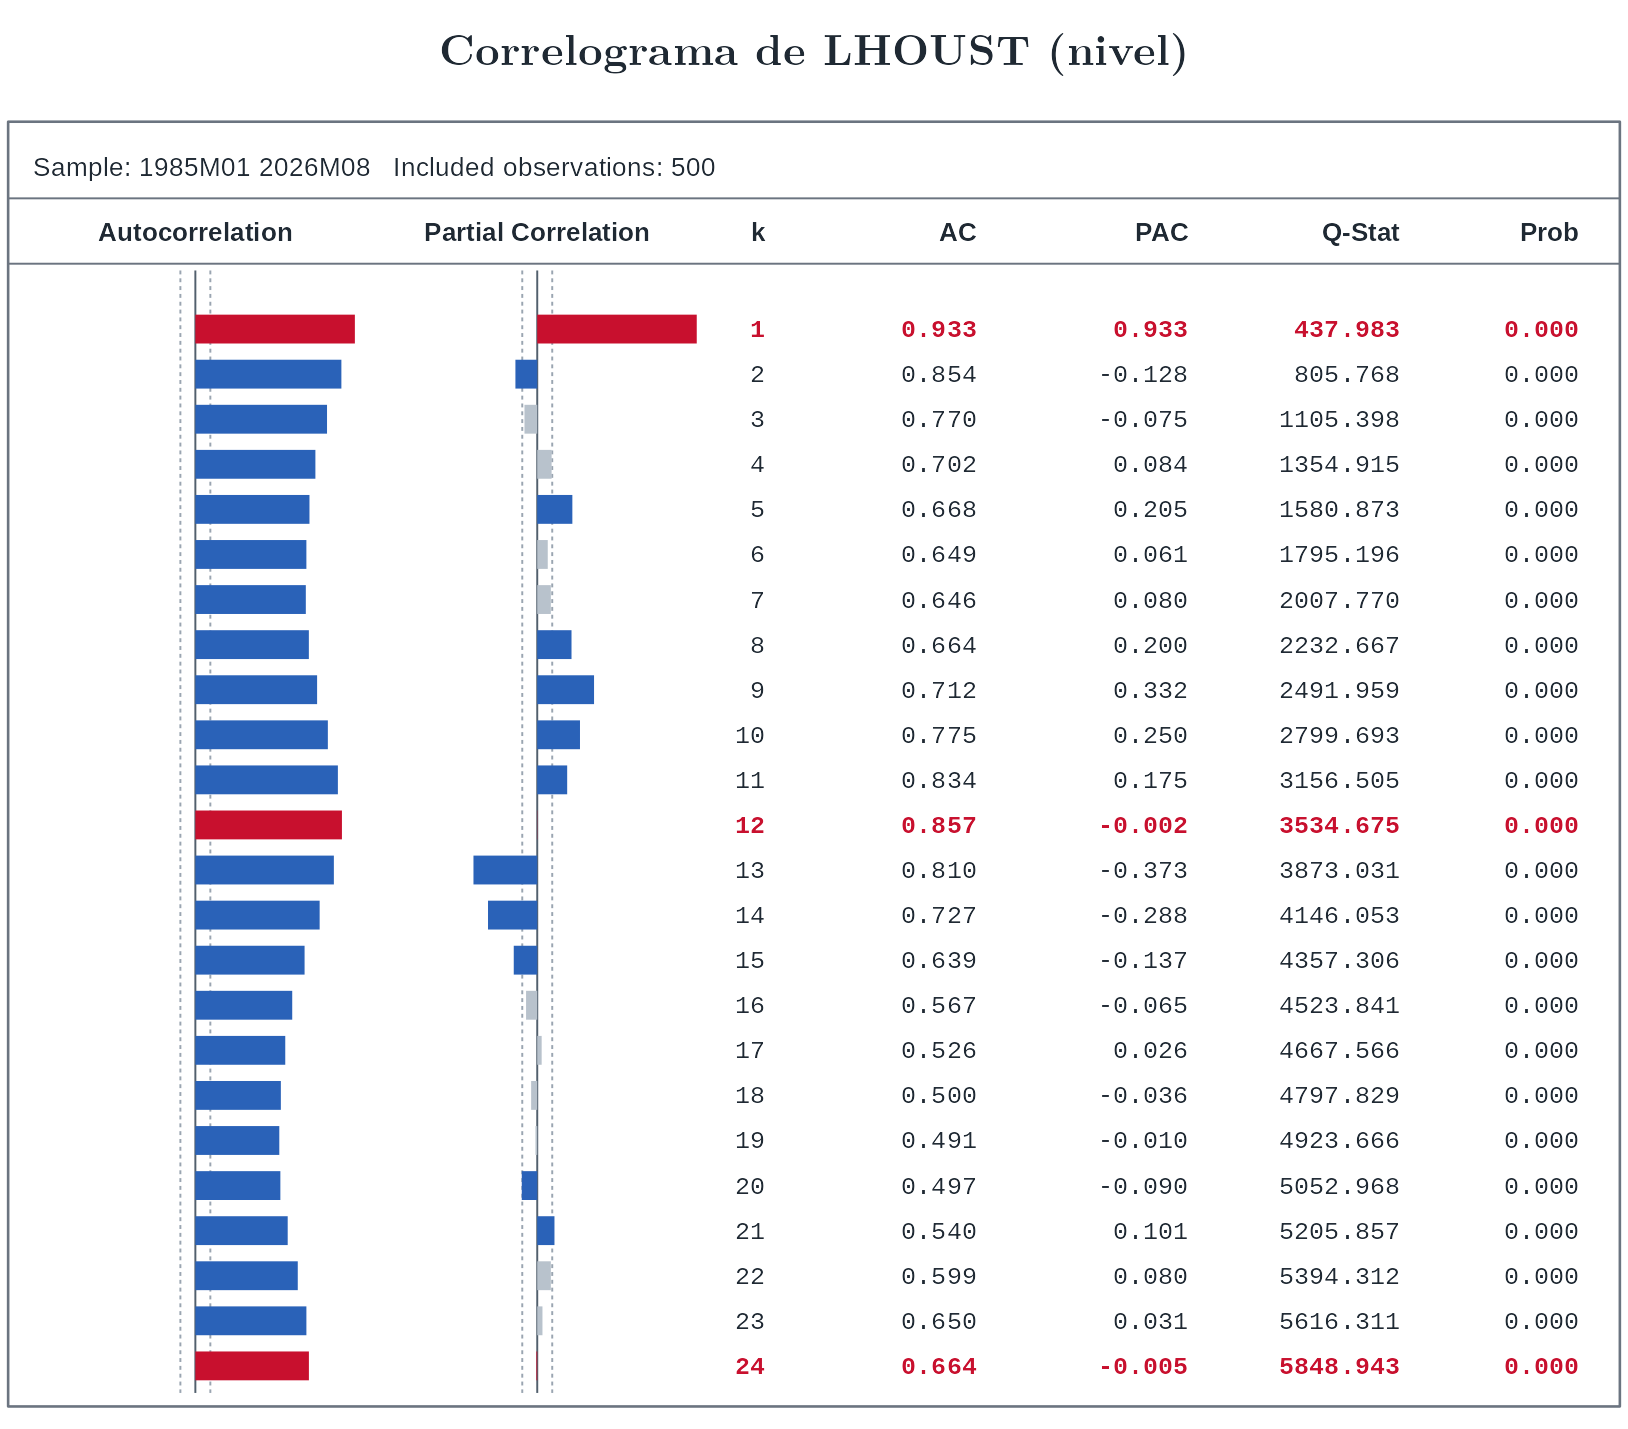
\includegraphics[width=0.49\linewidth]{03_corr_lhoust.png}\hfill
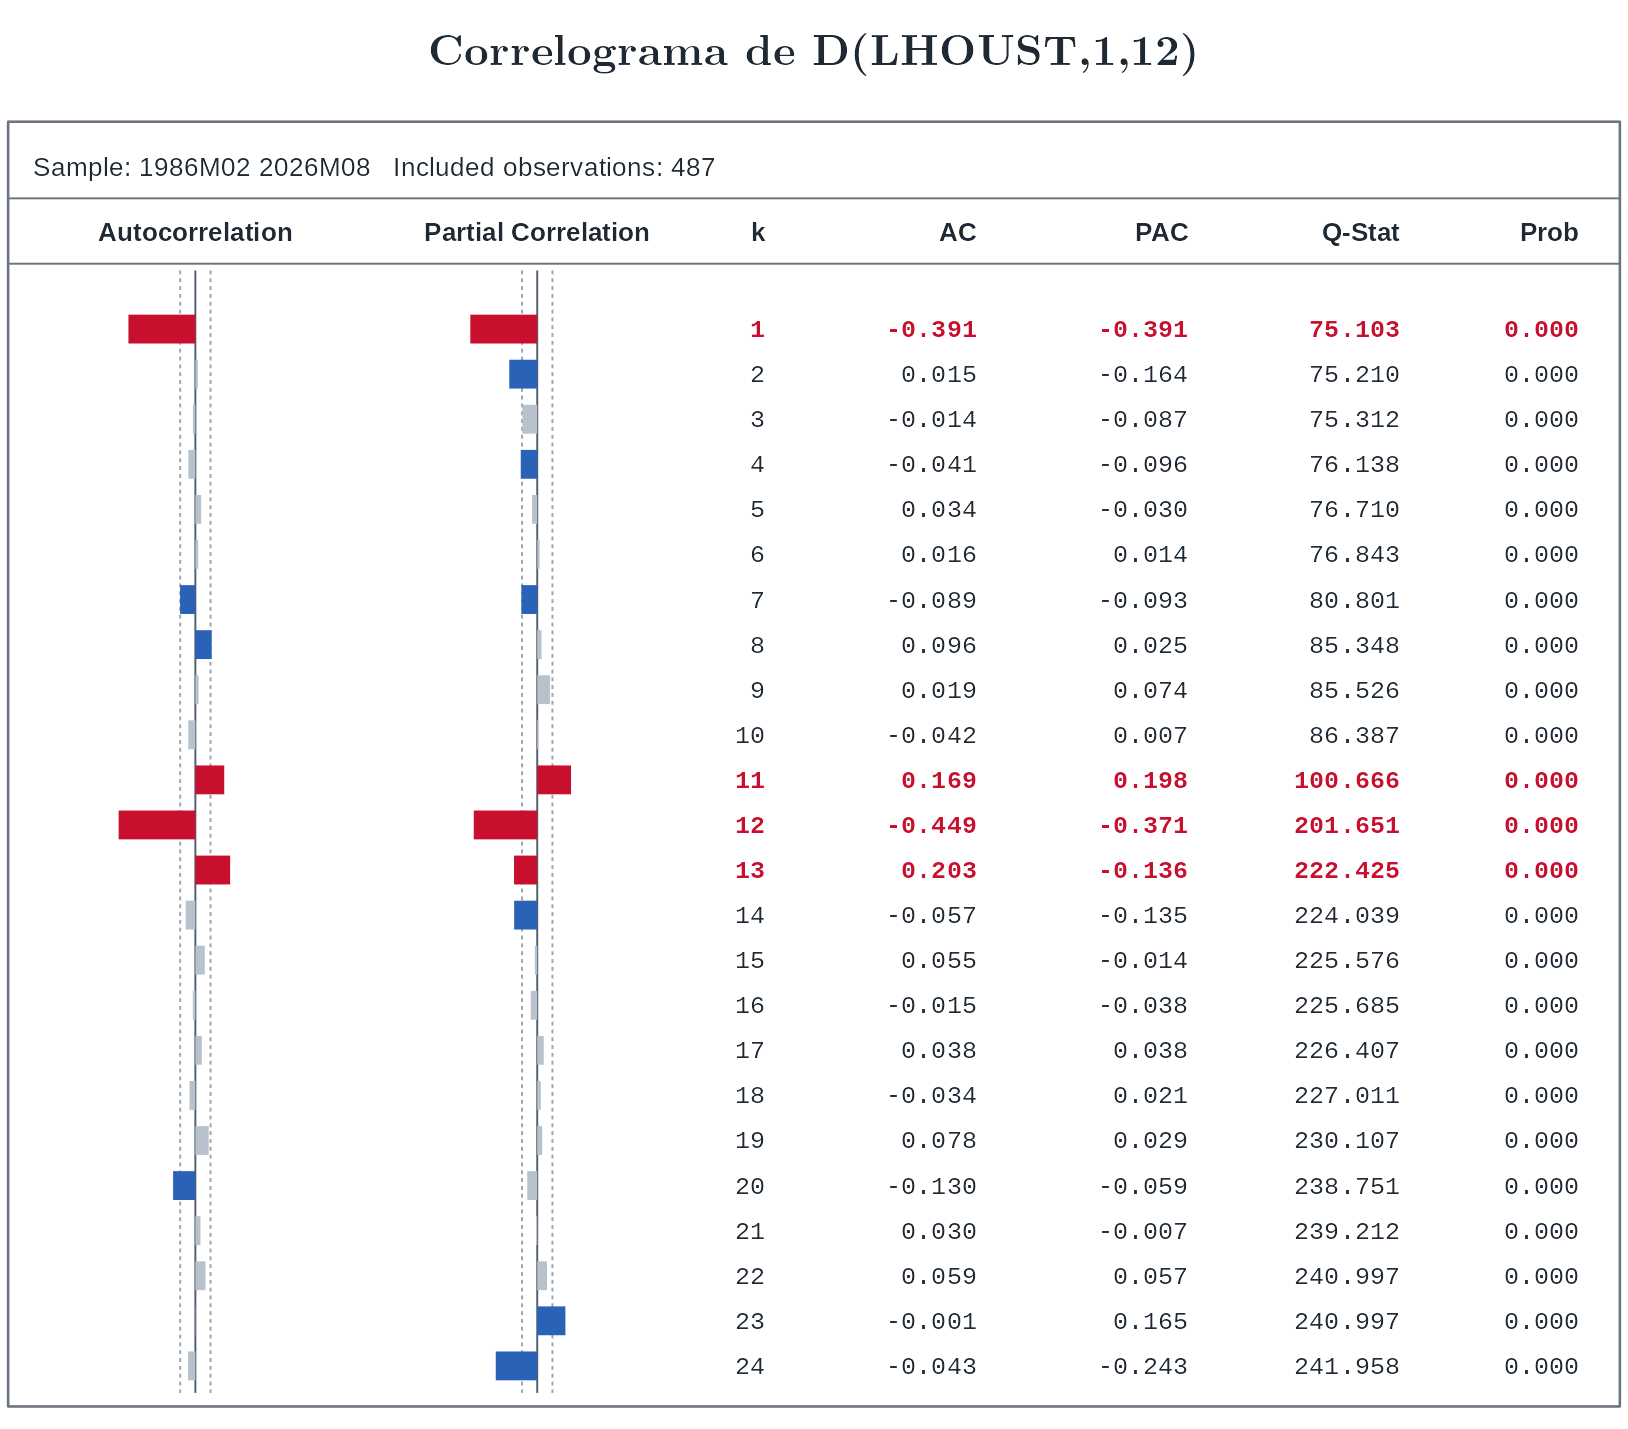
\includegraphics[width=0.49\linewidth]{03_corr_d112lhoust.png}
\caption{Correlogramas con $Q$ de Ljung--Box: inicios en nivel y con $(1-B)(1-B^{12})$.}
\end{figure}

\subsection{Dickey--Fuller aumentado}
Esquema descendente (Dickey--Pantula): primero $\Delta$, despu\'es el nivel ($\tau_\tau$, y $\tau_\mu$ si la tendencia no es significativa). 12 rezagos; sensibilidad con 24 y con SBC. $p$-valores de MacKinnon.
\tabla{03_adf.tex}{ADF, 1985--2026. Decisi\'on con 12 rezagos, al 5\%.}{tab:adf}
\begin{itemize}
\item \textbf{Ambas series $I(1)$:} se rechaza sobre la diferencia ($\AdfVivDif$, $\AdfTasaDif$) y no sobre el nivel ($\tau_\mu=\AdfVivNivTM$ y $\AdfTasaNivTM$; VC $\AdfVCtm$).
\item \textbf{El ADF no detecta la ra\'iz estacional} (solo testea $z=1$, \nota{6}{2.3}): la decide el correlograma.
\item \textbf{Sobre $(1-B^{12})x$ el ADF es fr\'agil:} $p=\AdfVivEstp$ con 12 rezagos, $p=\AdfVivEstSBCpv$ con SBC. Se aplica $(1-B)$: manda el correlograma (regla 6).
\end{itemize}
\salida{03_adf_lhoust.png}{0.6}{ADF del nivel de los inicios. Resto en el Ap\'endice~A.}

\subsection{Elecci\'on del filtro por SBC}
Mismas fechas (desde 1986-02); los SBC son comparables porque todo $F(B)$ con $F(0)=1$ tiene jacobiano unitario.
\tabla{04_filtros.tex}{Mejor modelo admisible por filtro.}{tab:filtros}
\begin{itemize}
\item \textbf{Gana $(1-B)(1-B^{12})$}: $\FiltroDSBCdos$ puntos sobre F2 y $\FiltroDSBCuno$ sobre dummies fijas.
\item F2 necesita un AR(1) con ra\'iz $\FiltroDosRaizAR$: la ra\'iz unitaria que falta.
\end{itemize}

%======================================================================
\section{Inicios: ARIMA$(0,1,1)(0,1,1)_{12}$}\label{sec:inicios}

\subsection{Identificaci\'on}
Rejilla de $\RejillaN$ modelos ARMA$(p\le3,q\le2)(P\le1,Q\le1)_{12}$ sobre $W_t=(1-B)(1-B^{12})x_t$; $\RejillaAdm$ admisibles. Gana por SBC el que sugiere el correlograma.
\tabla{04_rejilla.tex}{Los ocho modelos de menor SBC.}{tab:rejilla}
\tabla{04_fac_teorica.tex}{FAC emp\'irica y te\'orica del modelo estimado.}{tab:facteo}

\subsection{Estimaci\'on}
\[
(1-B)(1-B^{12})\,x_t=\omega\,(1-B)(1-B^{12})\,I_t^{2020.04}+(1-\theta B)(1-\Theta B^{12})\,a_t
\]
\begin{itemize}
\item $\hat\theta=\ThetaV$ (ee $\ThetaVee$), $\hat\Theta=\SThetaV$ (ee $\SThetaVee$), $\hat\sigma_a=\SigmaV\%$. Signo de las Notas; la salida usa $+\theta$.
\item AO: $\hat\omega=\AOV$ (ee $\AOVee$), es decir, $\AOVpct\%$.
\item Invertible: ra\'iz MA $\RaizMAV$; ra\'ices estacionales de m\'odulo $\RaizSMAV$.
\end{itemize}
\salida{04_modelo_inicios.png}{0.86}{Modelo de los inicios.}

\subsection{Diagn\'ostico}
\begin{itemize}
\item \textbf{Ljung--Box} ($K-2$ gl): $p=\LBVdoce$ / $\LBVveinticuatro$ / $\LBVtreintayseis$. Ruido blanco.
\item \textbf{Jarque--Bera}: $\JBV$ ($p=\JBVp$). Sin el AO: $\JBVsinAO$, y 2020-04 es un residuo de $\ResidAbrSinAO$ desv\'ios.
\item \textbf{Sobreajuste}: nada significativo ($|t|\le\SobreMaxT$); todo empeora el SBC.
\item \textbf{Cuadrados}: $p\ \LBcuadV$. Varianza no constante (limitaci\'on).
\end{itemize}
\begin{figure}[H]\centering
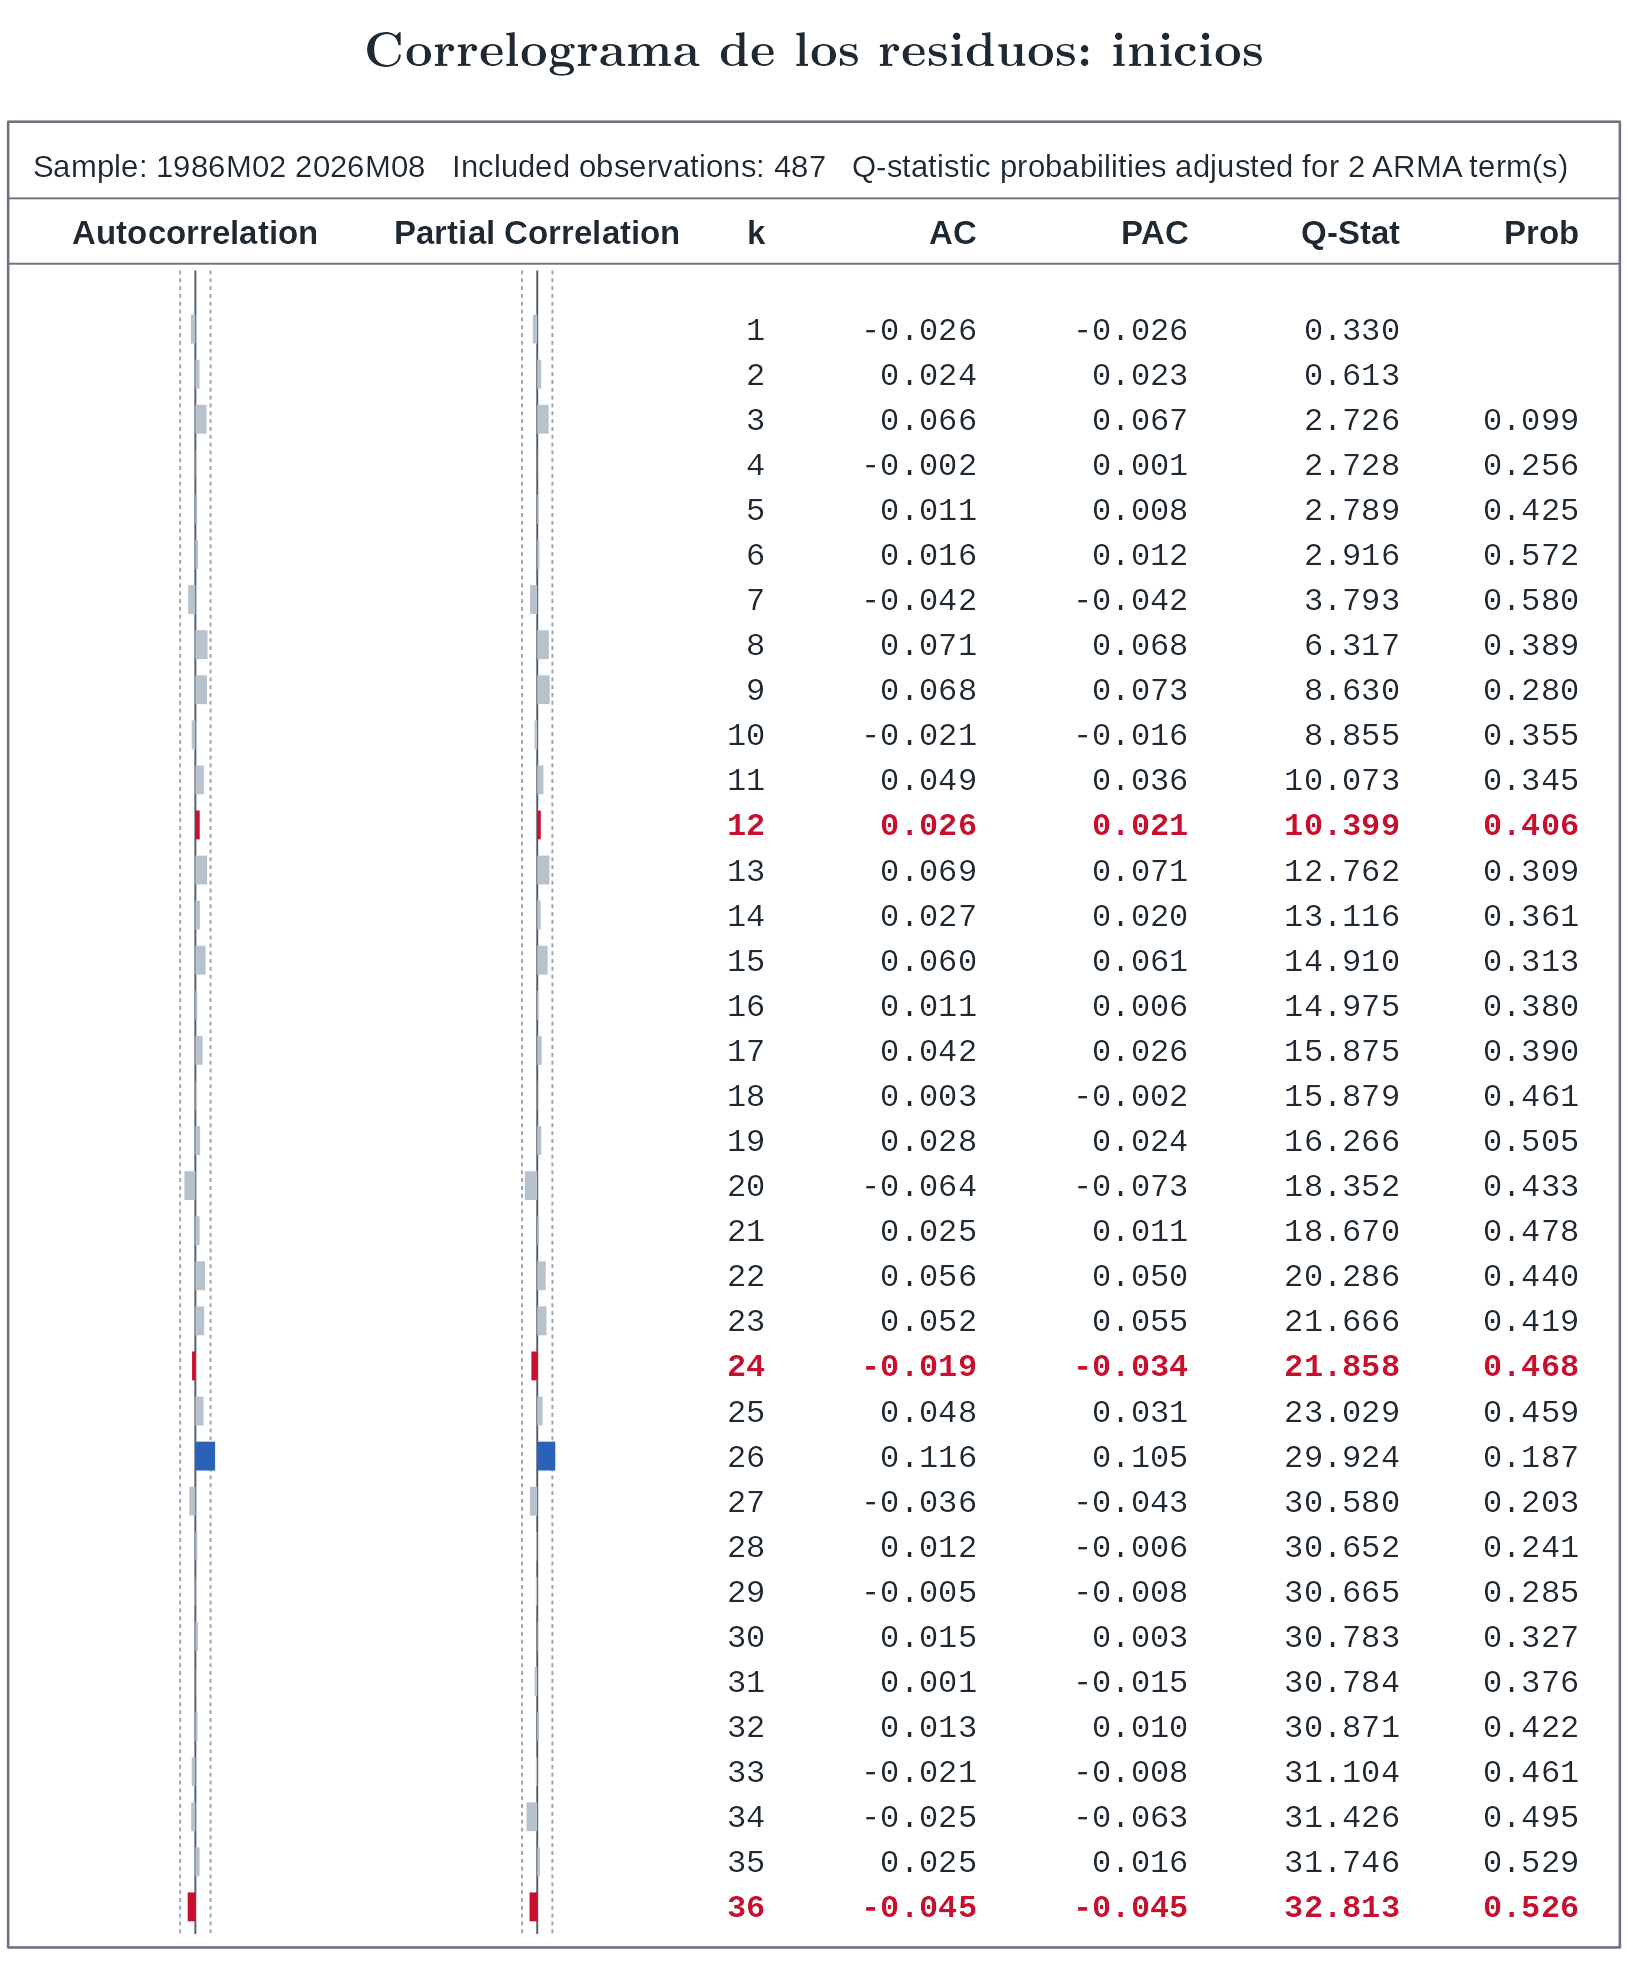
\includegraphics[width=0.56\linewidth]{04_corr_residuos.png}\hfill
\begin{minipage}[b]{0.42\linewidth}\small\begin{adjustbox}{max width=\linewidth}\begin{tabular}{lccc}
\toprule
Par\'ametro agregado & Estimaci\'on & $t$ & $\Delta$SBC
\\ \midrule
AR(1) & \ensuremath{-}0{,}113 & \textcolor{red}{\ensuremath{-}1{,}22} & 4{,}8 \\
MA(2) & 0{,}064 & \textcolor{red}{1{,}32} & 4{,}4 \\
SAR(12) & 0{,}045 & \textcolor{red}{0{,}84} & 5{,}5 \\
SMA(24) & \ensuremath{-}0{,}039 & \textcolor{red}{\ensuremath{-}0{,}85} & 5{,}5 \\
\bottomrule
\end{tabular}
\end{adjustbox}\par\vspace{6pt}
\captionof{table}{Sobreajuste \nota{6}{10.4}.}\end{minipage}
\caption{Correlograma de los residuos (ajustado por 2 t\'erminos ARMA).}
\end{figure}
\salida{04_residuos.png}{1}{Residuos estandarizados, FAC y Q--Q.}

\subsection{Estabilidad y serie desestacionalizada}\label{sec:estab}
\tabla{04_estabilidad.tex}{El modelo por subper\'iodos (regla 9).}{tab:estab}
\begin{itemize}
\item \textbf{Din\'amica estable:} $\hat\theta$ $\ThetaSubUno\to\ThetaSubDos$, $\hat\Theta$ $\SThetaSubUno\to\SThetaSubDos$. Sube $\hat\sigma$: $\SigmaSubUno\to\SigmaSubDos$.
\item \textbf{Desestacionalizada (regla 8):} conserva $\rho_{12}=\RhoSAdoce$; su mejor modelo, \SAmodelo, necesita parte estacional. Se descarta (Ap\'endice~A).
\end{itemize}

%======================================================================
\section{Tasa: ARIMA(0,1,1)}\label{sec:tasa}
\begin{figure}[H]\centering
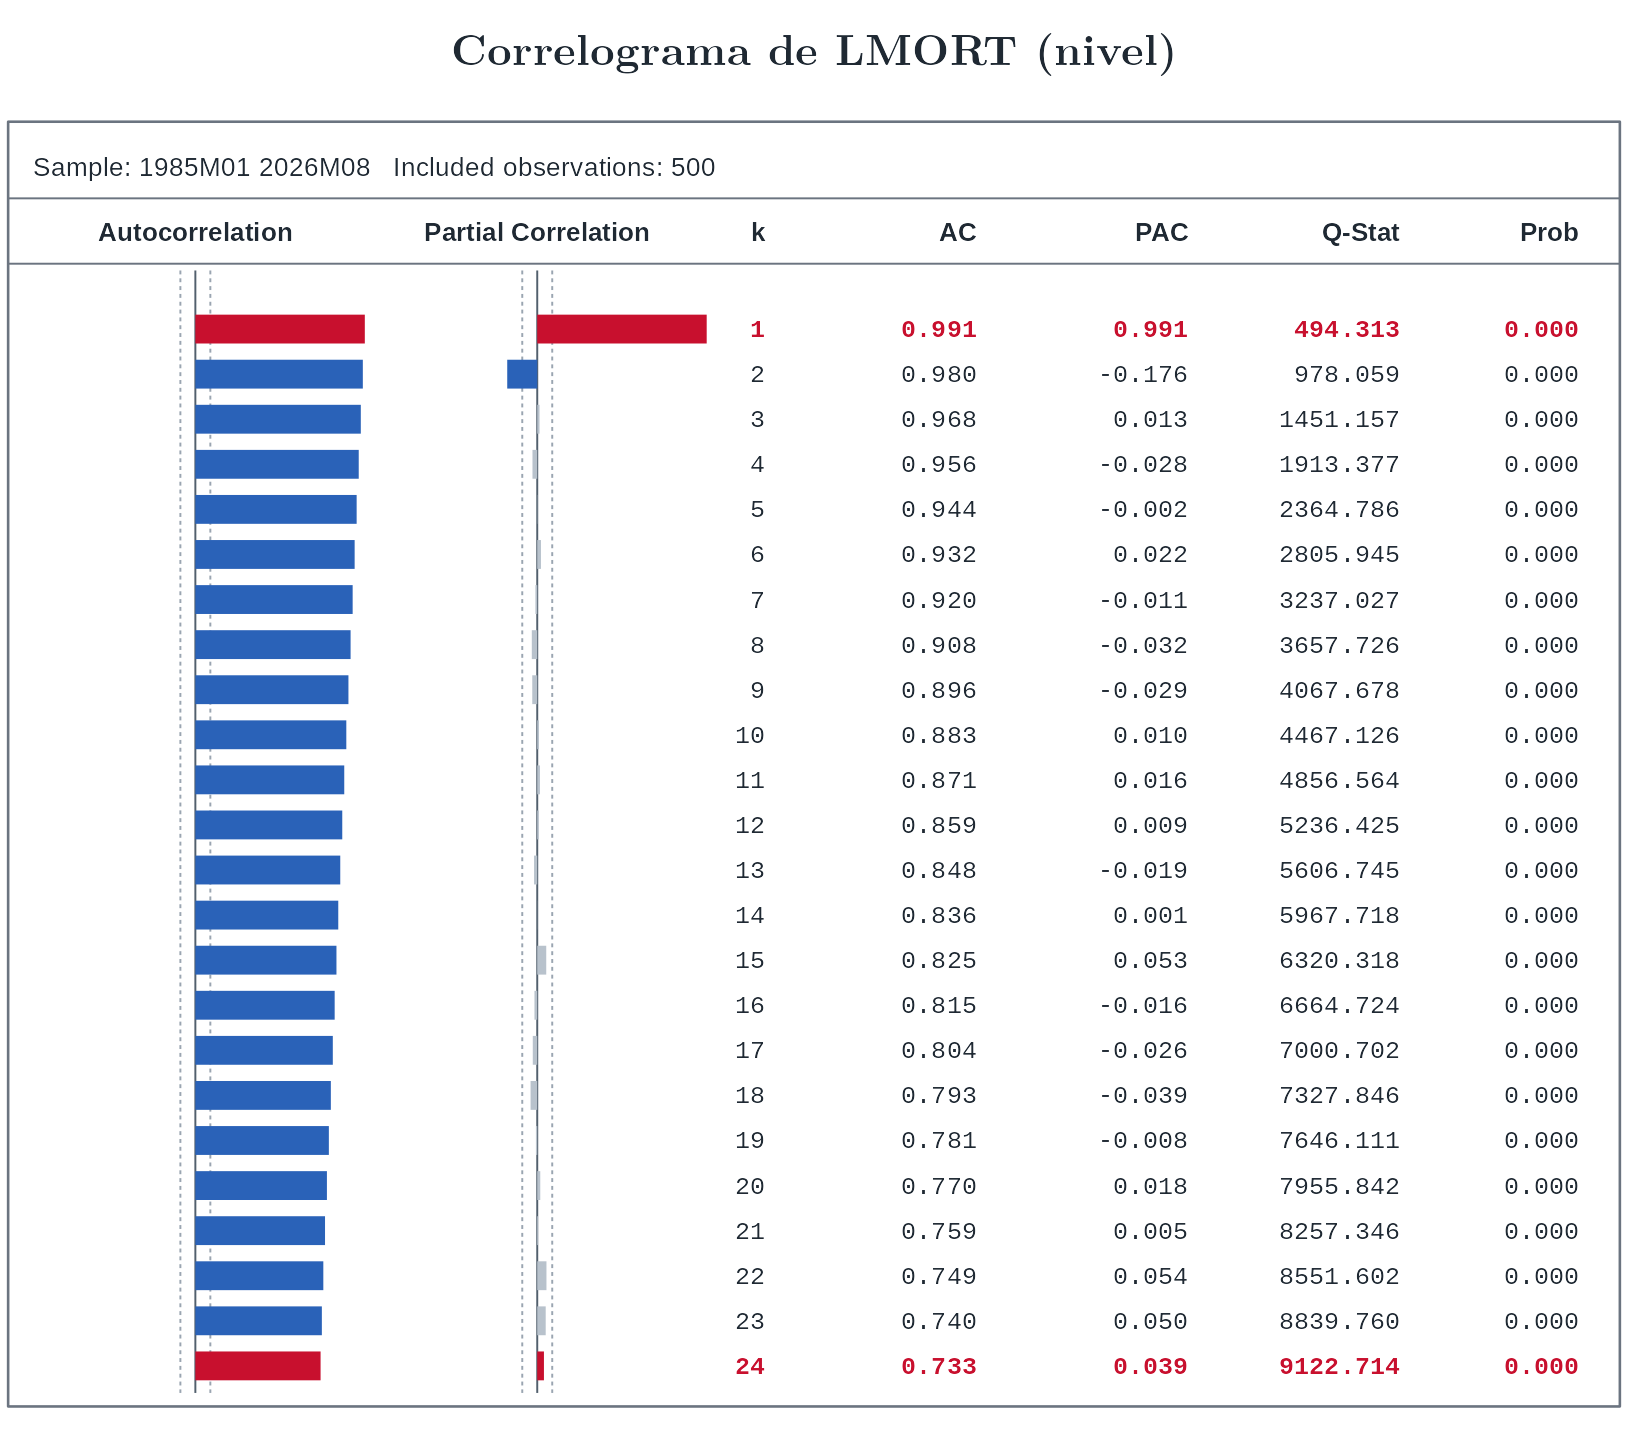
\includegraphics[width=0.49\linewidth]{03_corr_lmort.png}\hfill
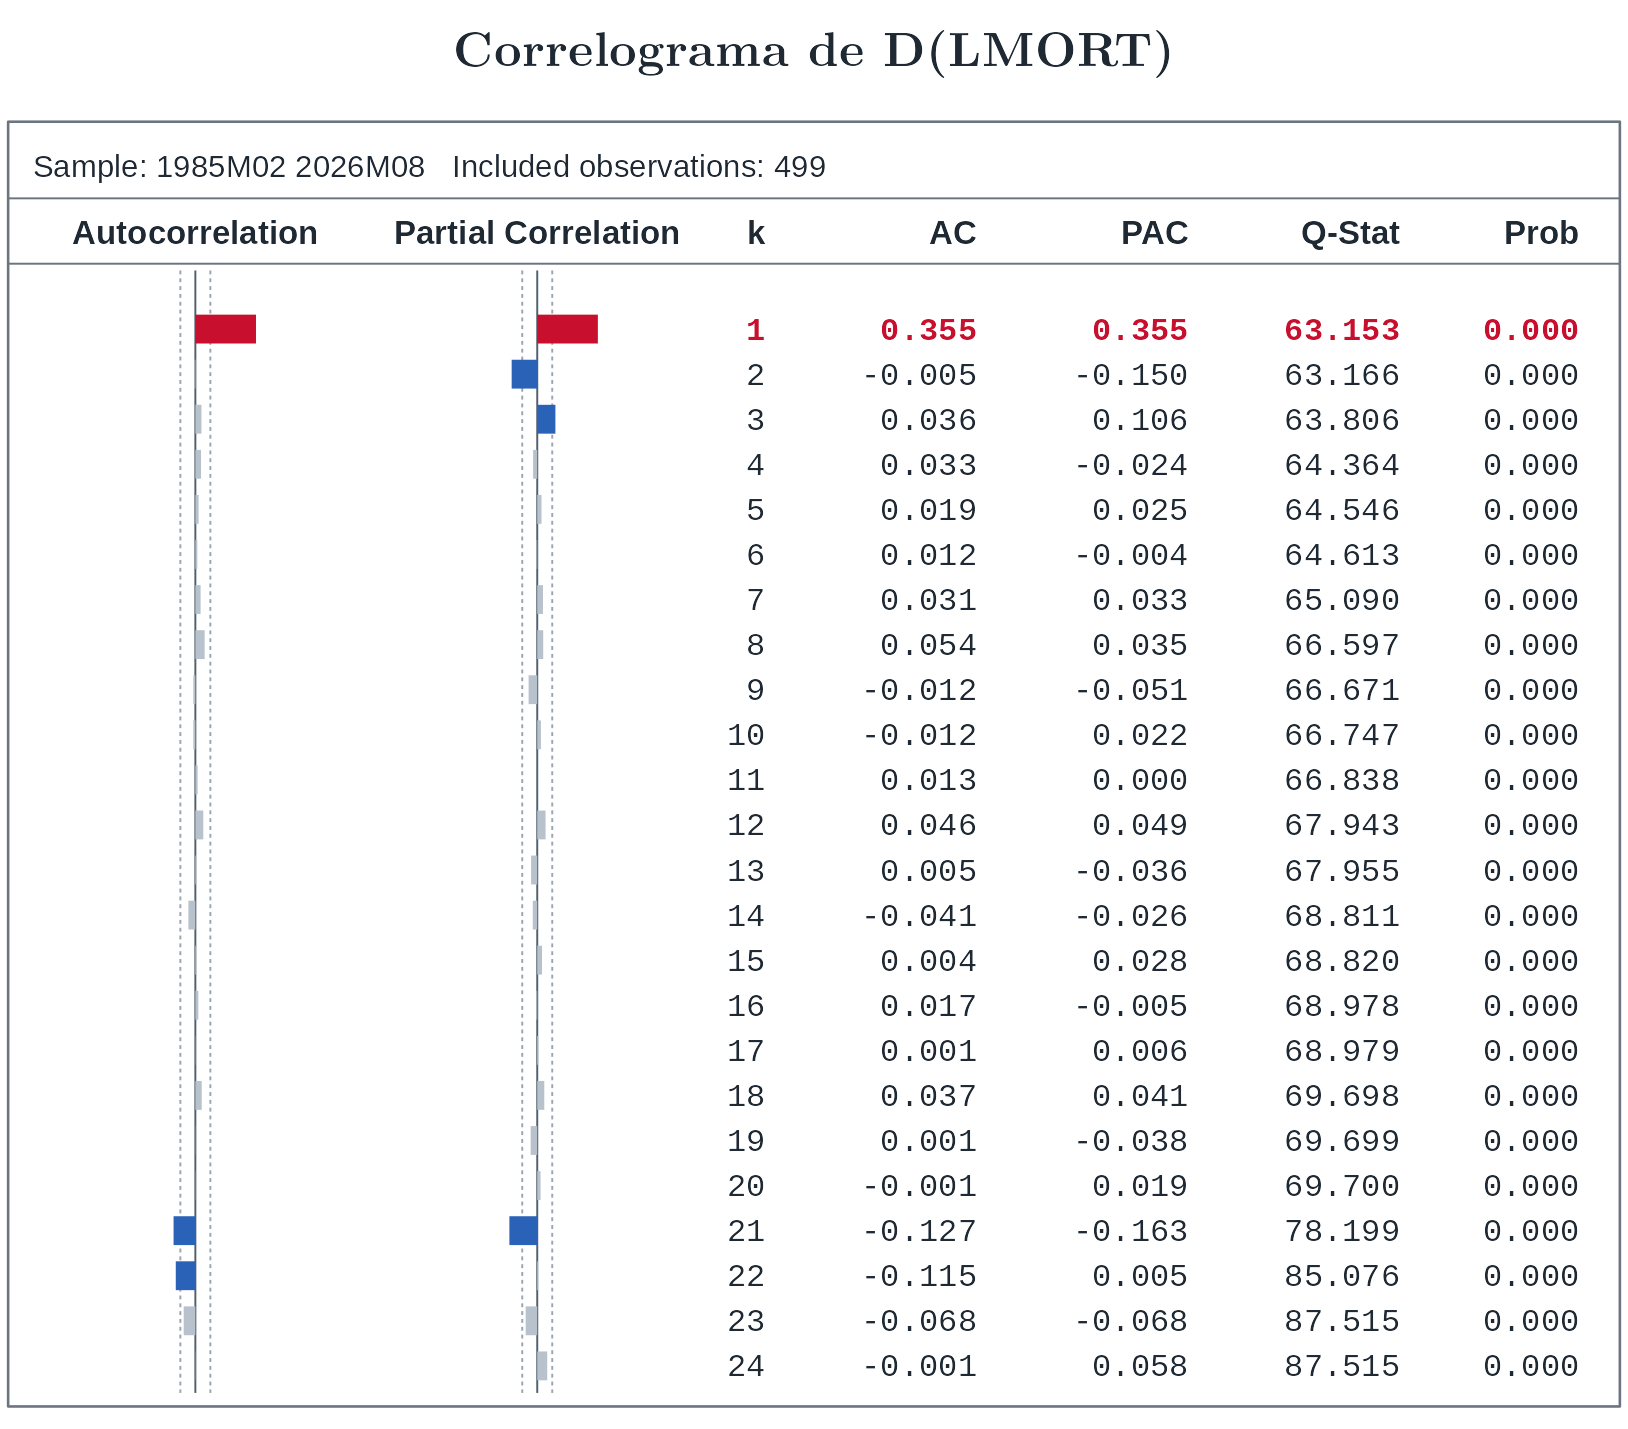
\includegraphics[width=0.49\linewidth]{03_corr_dlmort.png}
\caption{Correlogramas de la tasa: nivel y primera diferencia.}
\end{figure}
\tabla{05_rejilla.tex}{Los ocho modelos de menor SBC sobre $(1-B)y_t$.}{tab:rejtasa}
\[
(1-B)\,y_t=(1-\theta B)\,a_t,\qquad \hat\theta=\ThetaT\ (\ThetaTee),\qquad \hat\sigma_a=\SigmaT\%
\]
\begin{itemize}
\item Sin constante (empeora el SBC). $\hat\theta<0$ $\Rightarrow$ $\rho_1=\RhoTeoT$: inercia de un mes.
\item \textbf{Ljung--Box}: $p=\LBTdoce$ / $\LBTveinticuatro$ / $\LBTtreintayseis$. Sobreajuste y subper\'iodos confirman el MA(1).
\item \textbf{Limitaci\'on:} colas pesadas (curtosis $\CurtosisT$, JB $=\JBT$) y varianza cambiante (cuadrados: $p\ \LBcuadT$). Residuos extremos: $\AtipicosT$ (Fed compra MBS, \emph{taper tantrum}, suba de tasas 2022).
\end{itemize}
\salida{05_modelo_tasa.png}{0.86}{Modelo de la tasa.}
\begin{figure}[H]\centering
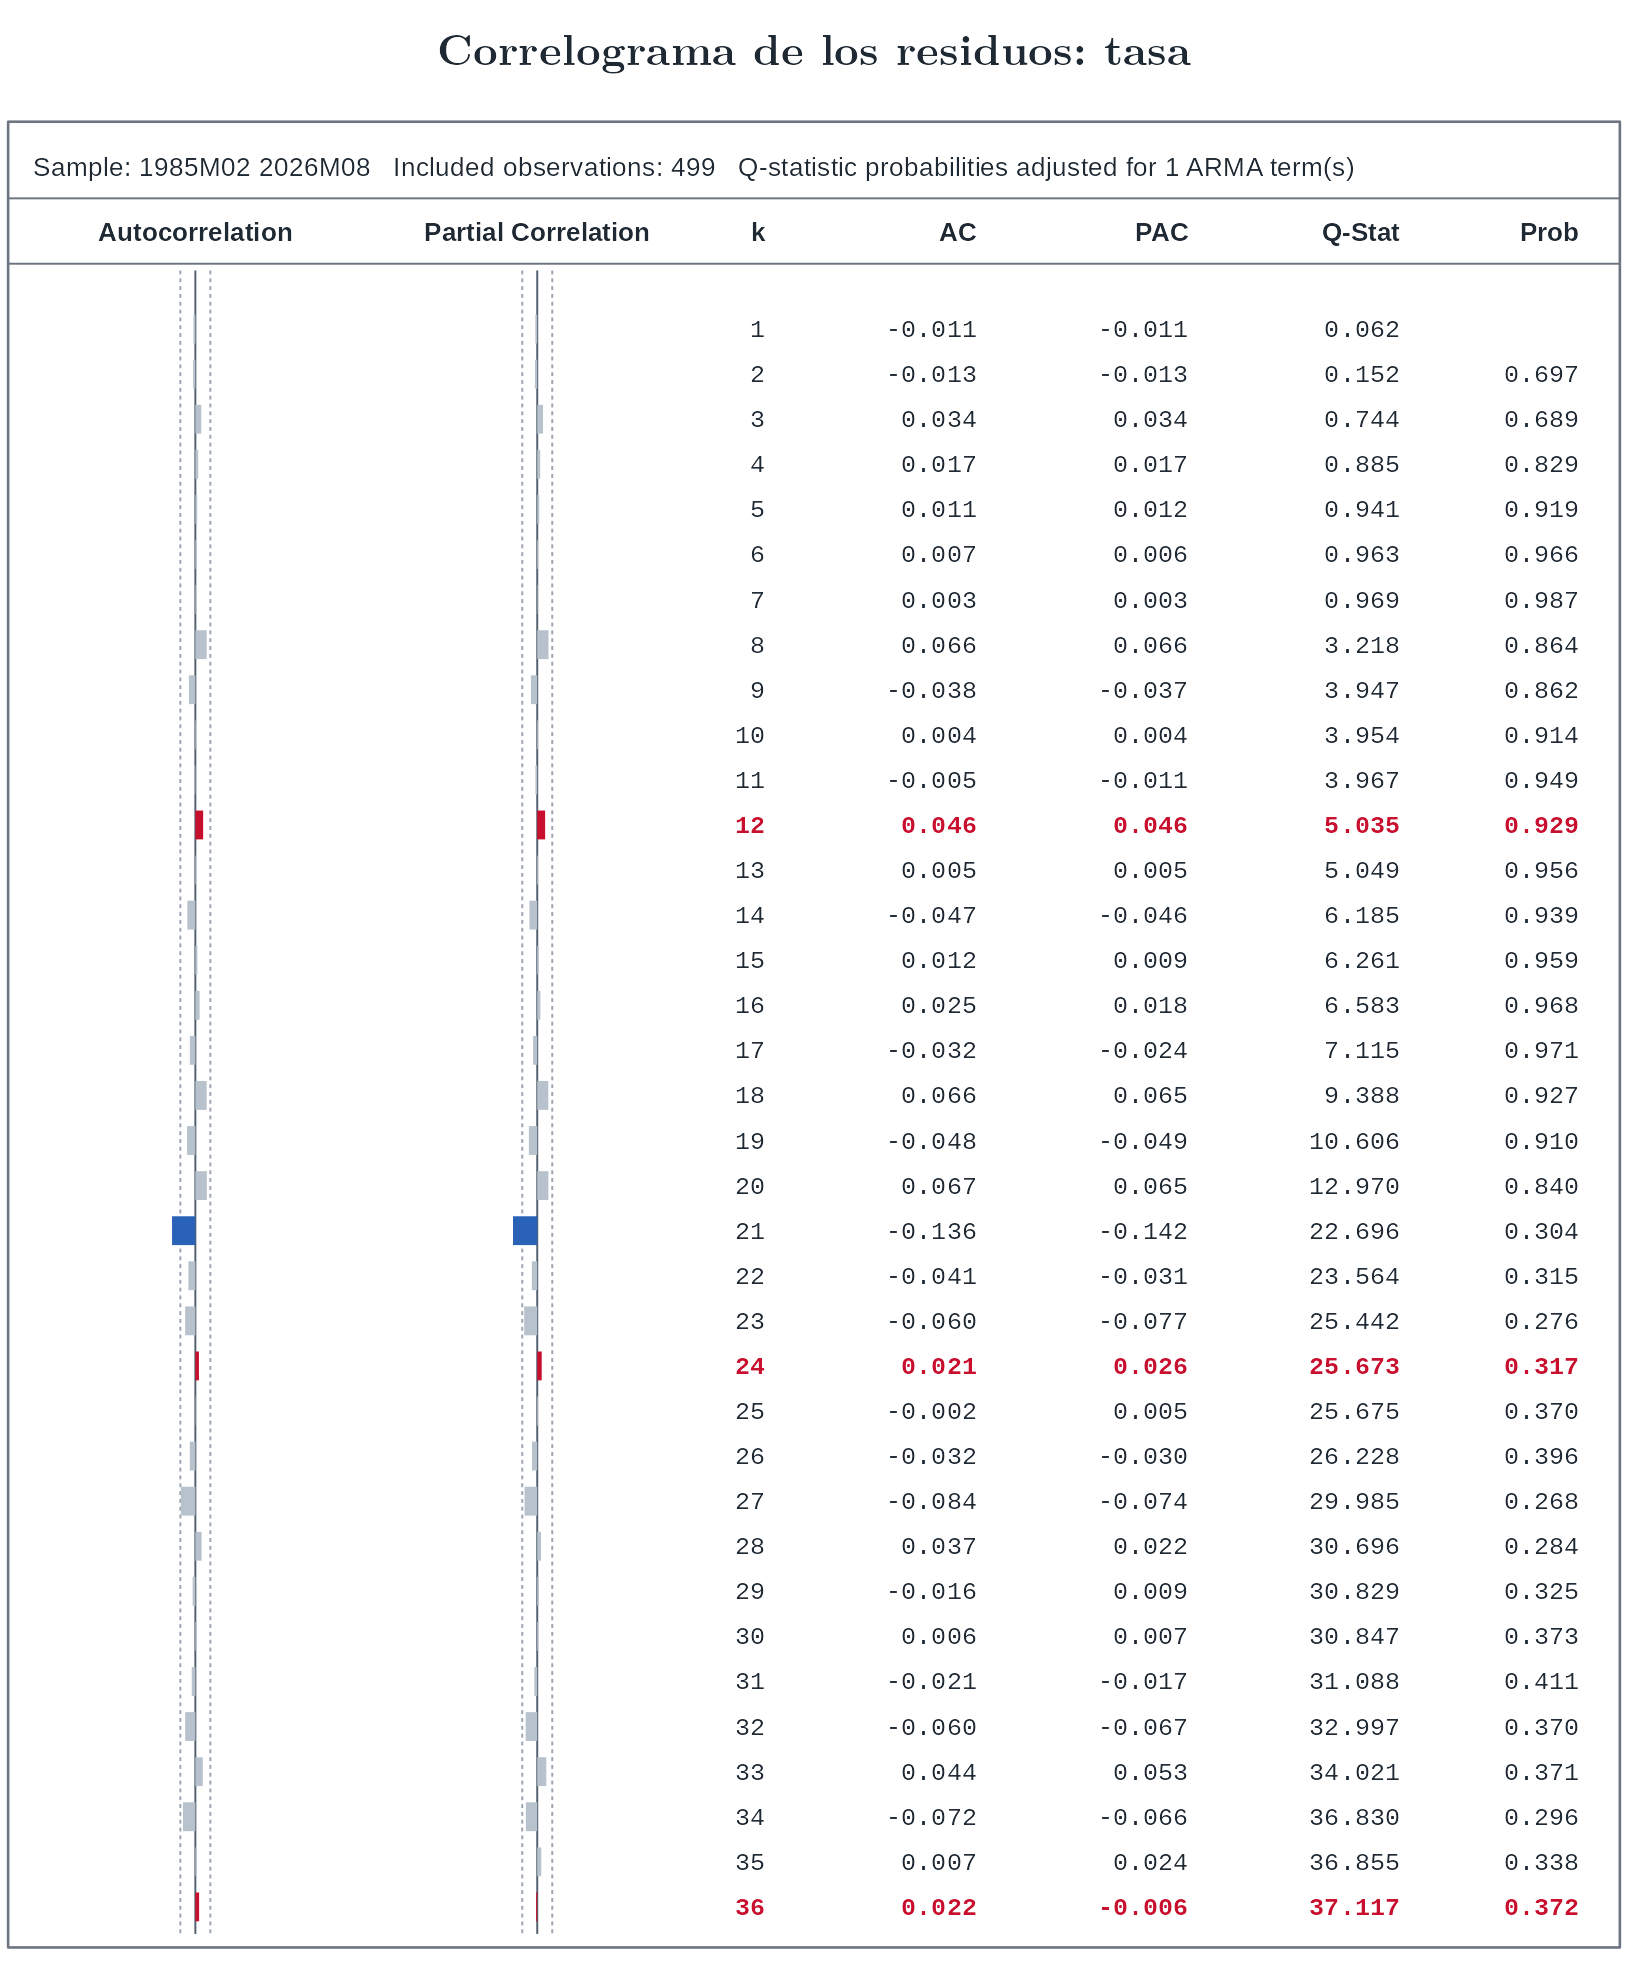
\includegraphics[width=0.56\linewidth]{05_corr_residuos.png}\hfill
\begin{minipage}[b]{0.42\linewidth}\small\begin{adjustbox}{max width=\linewidth}\begin{tabular}{lccc}
\toprule
Par\'ametro agregado & Estimaci\'on & $t$ & $\Delta$SBC
\\ \midrule
AR(1) & \ensuremath{-}0{,}055 & \textcolor{red}{\ensuremath{-}0{,}55} & 5{,}9 \\
MA(2) & \ensuremath{-}0{,}023 & \textcolor{red}{\ensuremath{-}0{,}53} & 5{,}9 \\
\bottomrule
\end{tabular}
\end{adjustbox}\par\vspace{4pt}
\captionof{table}{Sobreajuste.}\par\vspace{8pt}
\begin{adjustbox}{max width=\linewidth}\begin{tabular}{lccc}
\toprule
Muestra & $\hat\theta$ (ee) & $\hat\sigma$ & $n$
\\ \midrule
1985--2026 (modelo elegido) & \ensuremath{-}0{,}44 (0{,}04) & 3{,}13 & 499 \\
1985--2007 & \ensuremath{-}0{,}46 (0{,}05) & \textcolor{red}{2{,}56} & 275 \\
2008--2026 & \ensuremath{-}0{,}43 (0{,}06) & \textcolor{red}{3{,}72} & 224 \\
\bottomrule
\end{tabular}
\end{adjustbox}\par\vspace{4pt}
\captionof{table}{Subper\'iodos.}\end{minipage}
\caption{Correlograma de los residuos de la tasa (ajustado por 1 t\'ermino ARMA).}
\end{figure}
\salida{05_residuos.png}{1}{Residuos de la tasa.}

%======================================================================
\section{Pron\'ostico fuera de muestra}
Estimaci\'on 1985--2017, evaluaci\'on 2018--2019 ($\NEval$ or\'igenes m\'oviles, $h=1,3,6,12$). Orden elegido solo con la muestra de estimaci\'on (coincide con el final).
\tabla{06_metricas_inicios.tex}{Inicios: RMSE (\%) y MAPE (\%, sobre el nivel); $U$ de Theil a un paso.}{tab:pronv}
\tabla{06_metricas_tasa.tex}{Tasa: RMSE (\%) y MAPE (\%).}{tab:pront}
\begin{itemize}
\item \textbf{Inicios:} mejora sobre el paseo aleatorio estacional de $\MejoraUno$, $\MejoraTres$, $\MejoraSeis$ y $\MejoraDoce\%$. A 12 meses empata con el ingenuo estacional. Combinar con F2 no agrega.
\item \textbf{Tasa:} mejora $\MejoraTasaUno\%$ a un mes y nada a 12 (pron\'ostico plano tras el primer paso, \nota{6}{3.4}).
\end{itemize}
\salida{06_pronostico.png}{0.85}{Arriba: desde 2017-12 contra lo observado ($\CoberturaAbanico\%$ dentro de la banda). Abajo: 12 meses desde 2026-08.}

%======================================================================
\section{Relaci\'on entre las series}\label{sec:relacion}

\subsection{Niveles: regresi\'on espuria}
\tabla{07_alarma.tex}{Regresiones de $\ln$ inicios sobre $\ln$ tasa.}{tab:alarma}
\begin{itemize}
\item \textbf{Niveles:} pendiente positiva ($t=\NivT$), signo equivocado; $d_W=\NivDW$. Con dummies, $R^2=\DumR>d_W=\DumDW$.
\item \textbf{Filtradas:} la relaci\'on contempor\'anea desaparece ($R^2=\FilR$).
\end{itemize}
\salida{07_reg_niveles.png}{0.72}{Regresi\'on en niveles.}

\subsection{Innovaciones: correlaci\'on cruzada y Haugh}
Residuos de los dos modelos univariados; banda $\pm\BandaCC$; $S=n\sum_{-M}^{M}r_k^2\sim\chi^2_{2M+1}$.
\salida{07_relacion.png}{1}{Izquierda: correlaci\'on cruzada de las innovaciones. Derecha: respuesta acumulada.}
\tabla{07_haugh.tex}{Test de Haugh. Las dos \'ultimas columnas separan la direcci\'on ($M=12$).}{tab:haugh}
\begin{itemize}
\item \textbf{No son independientes} ($M=6$: $p\ \HaughSeisP$).
\item \textbf{Direcci\'on:} en toda la muestra domina tasa $\to$ inicios ($k>0$: $p=\HaughDocePos$), con correlaciones negativas a 3, 5 y 6 meses.
\item \textbf{Retroalimentaci\'on:} inicios $\to$ tasa no es significativa en conjunto ($k<0$: $p=\HaughDoceNeg$), pero $r_{-1}=0{,}15$ s\'i lo es, y en 1986--2007 la direcci\'on es significativa ($p=0{,}043$).
\end{itemize}

\subsection{Rezagos distribuidos con el mismo filtro}
$F(B)=(1-B)(1-B^{12})$ en ambas series: $F(B)x_t=v(B)F(B)y_t+F(B)n_t$, con $v(B)$ intacto. MCO con rezagos 0--12 y el AO.
\salida{07_reg_rezagos.png}{0.8}{Rezagos distribuidos 0--12 (elasticidades).}
\tabla{07_respuesta.tex}{Elasticidad acumulada. Tercera columna: efecto de +1\,pp sobre $\TasaUltima\%$ ($+\PPequiv\%$ de la tasa).}{tab:resp}
\begin{itemize}
\item \textbf{Elasticidad:} $\ElasTres$ (ee $\ElasTresee$) a 3 meses, $\ElasDoce$ (ee $\ElasDoceee$) a 12.
\item \textbf{En puntos:} +1\,pp $\Rightarrow$ $\PPDoce\%$ de inicios a un a\~no; IC 95\% $[\PPDoceLo\%;\ \PPDoceHi\%]$.
\item Errores est\'andar orientativos ($d_W=\RDdw$): corresponde funci\'on de transferencia (segunda parte).
\end{itemize}

%======================================================================
\section{Limitaciones y pasos siguientes}
\begin{itemize}
\item \textbf{Exogeneidad:} hay retroalimentaci\'on de corto plazo (inicios $\to$ tasa a un mes). Opciones: VAR, que trata a ambas como end\'ogenas, o el bono a 10 a\~nos como causa.
\item \textbf{Intervenciones:} 2020-04 (inicios); 2008-12, 2013-06 y 2022 (tasa).
\item \textbf{Varianza:} heterocedasticidad en ambas series; colas pesadas en la tasa.
\item \textbf{Estacionalidad:} la ra\'iz estacional se decidi\'o por correlograma y SBC (HEGY fuera del programa).
\end{itemize}

\medskip\noindent\textit{Fuentes:} U.S.\ Census Bureau, Freddie Mac PMMS, FRED. Teor\'ia: Notas 1 a 6 y apunte de la c\'atedra.

%======================================================================
\appendix
\section{Salidas complementarias}
\begin{figure}[H]\centering
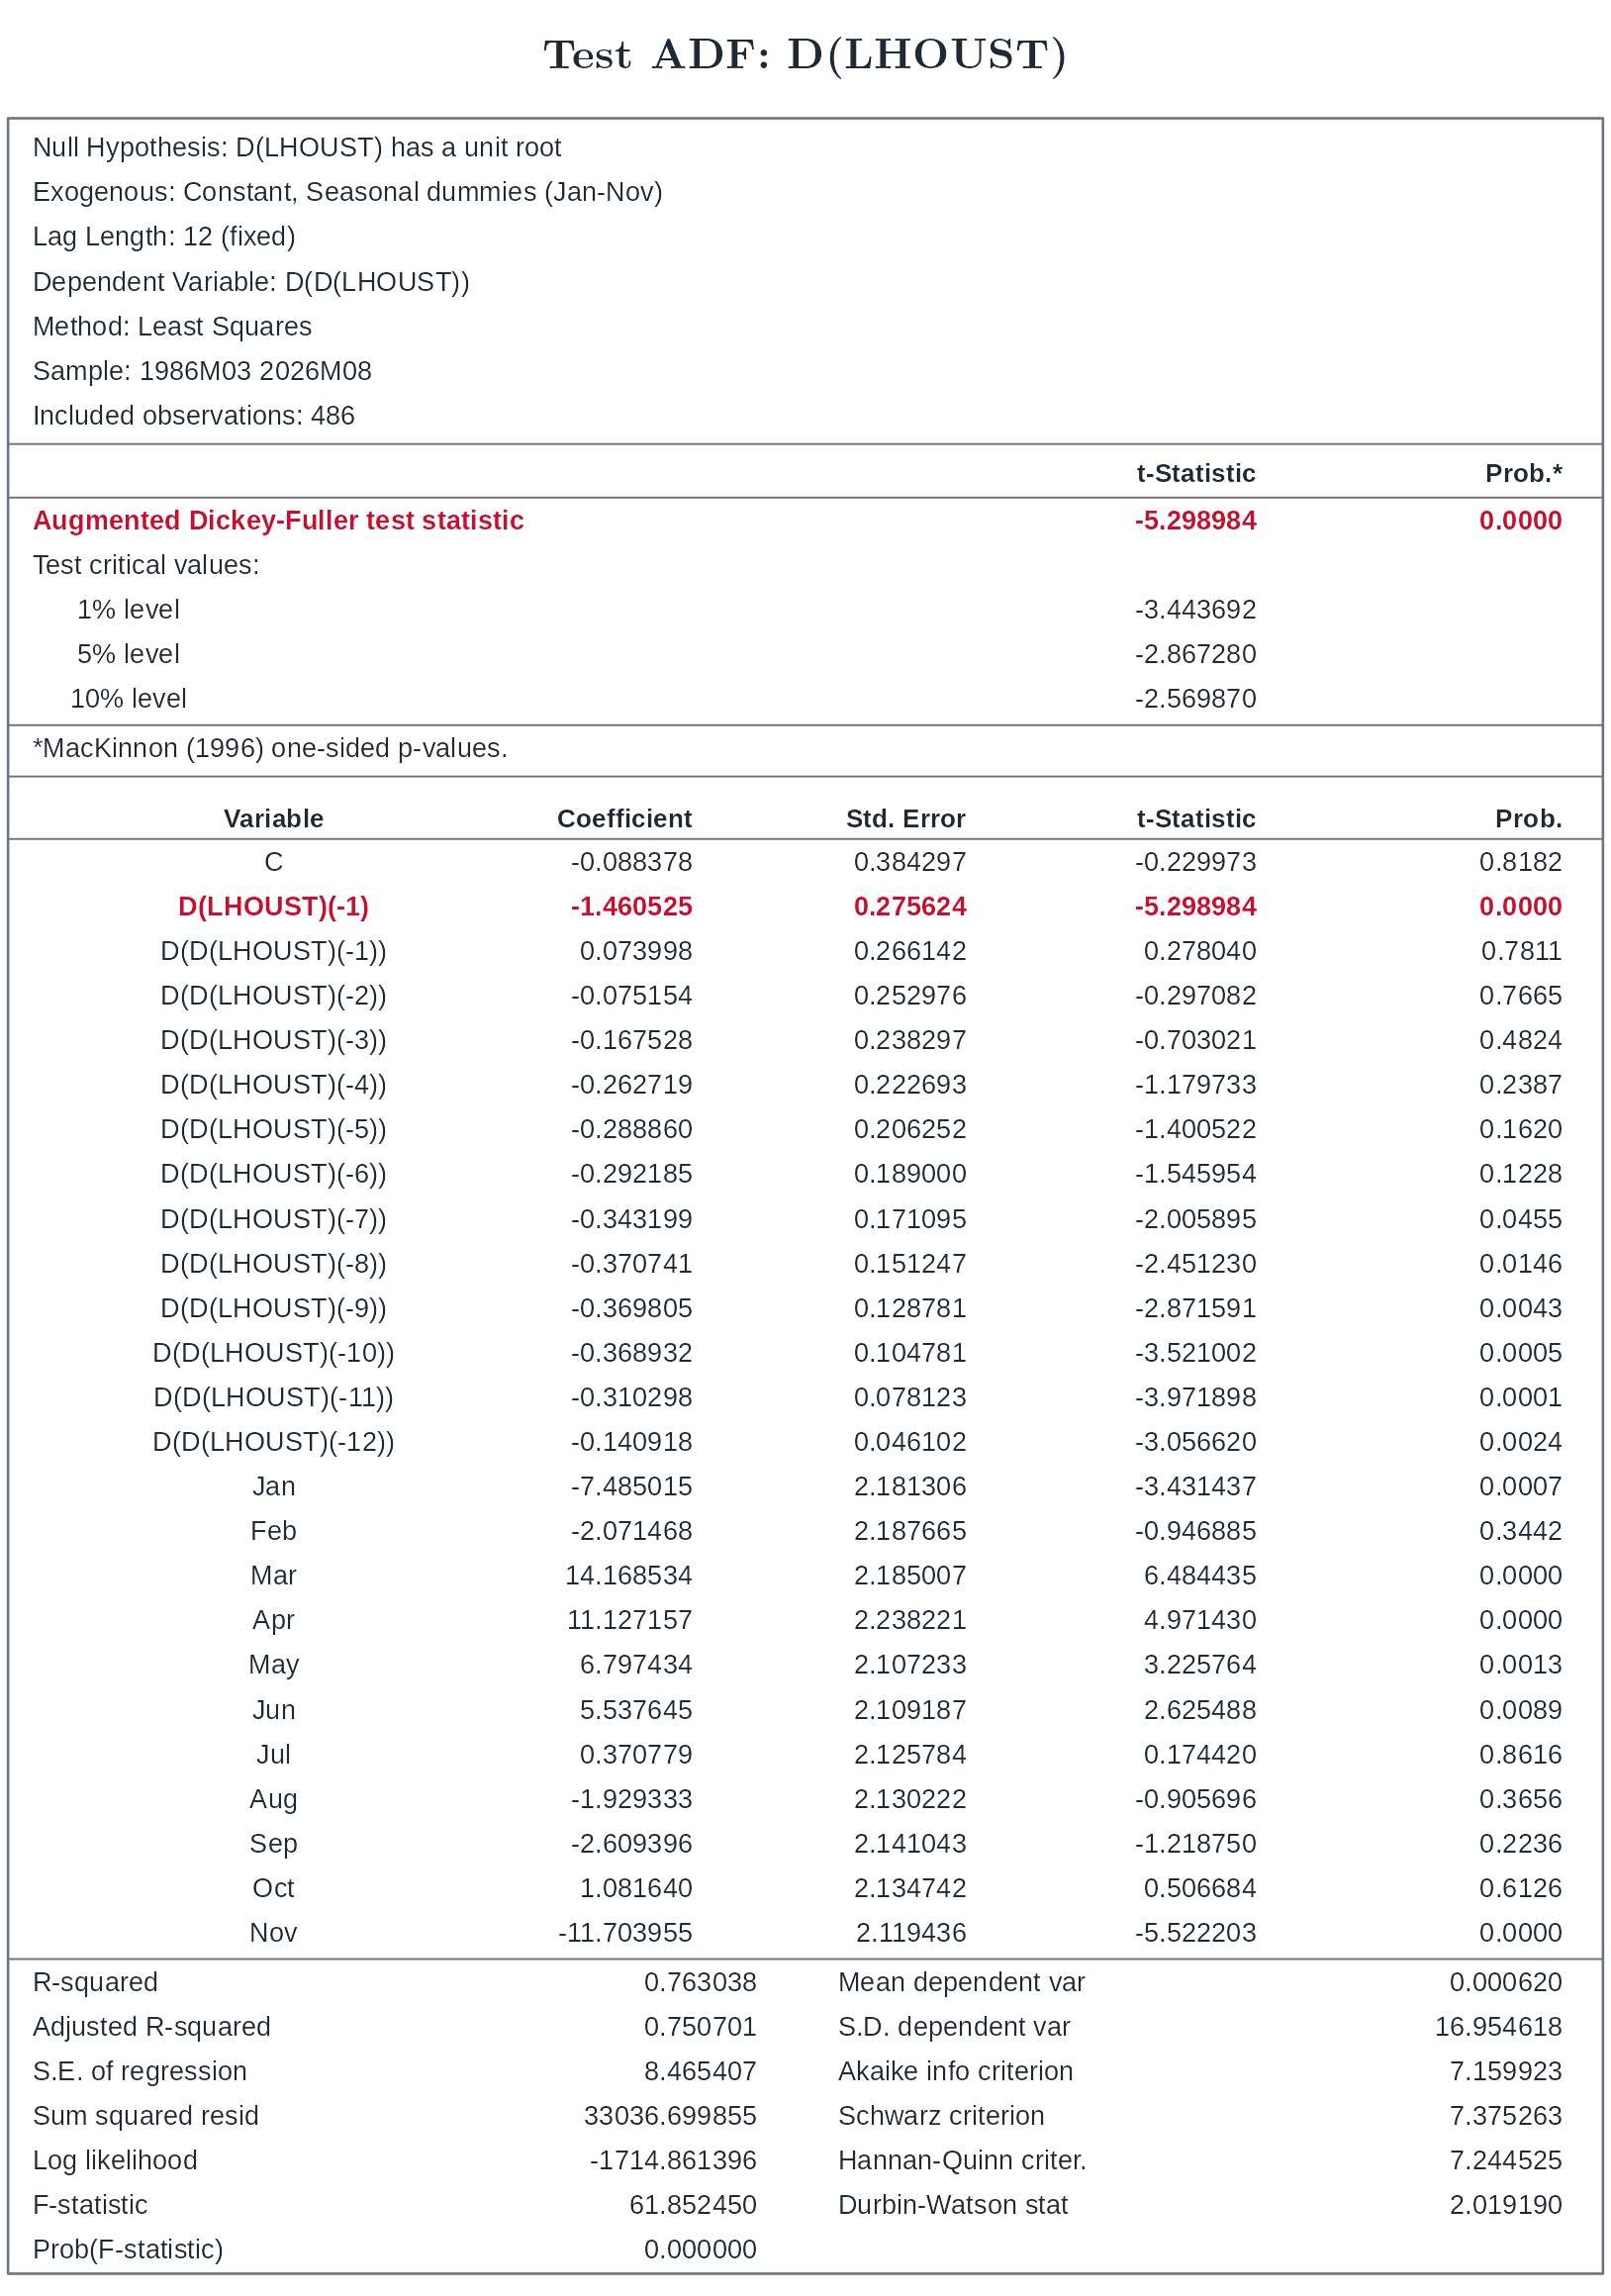
\includegraphics[width=0.49\linewidth]{03_adf_dlhoust.png}\hfill
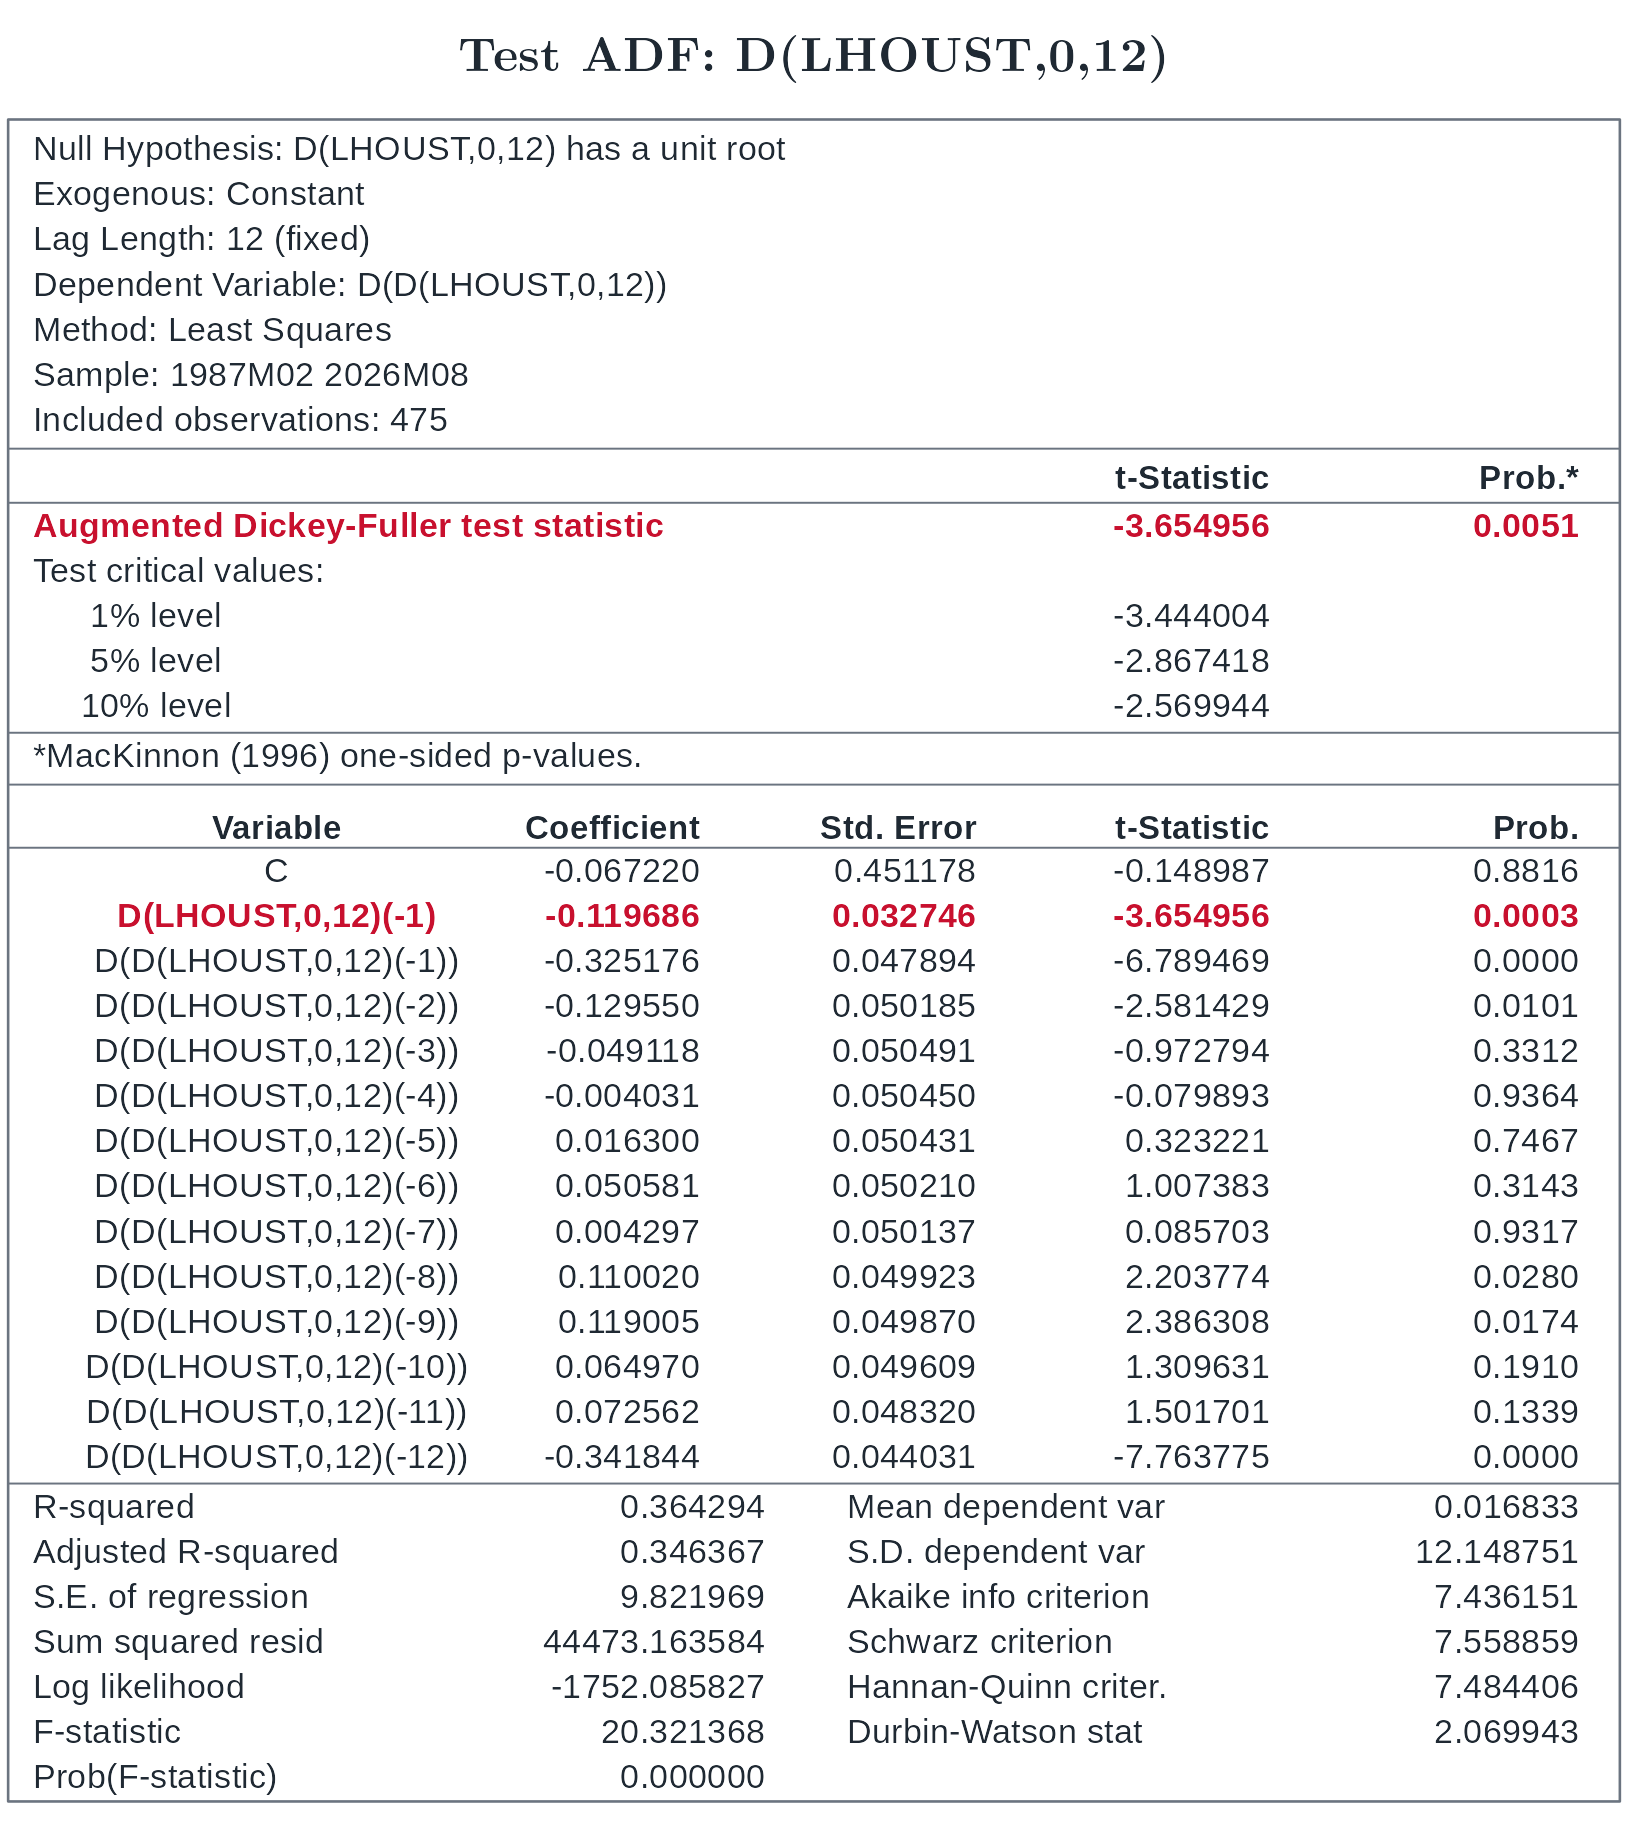
\includegraphics[width=0.49\linewidth]{03_adf_d12lhoust.png}
\caption{ADF sobre $\Delta x$ (paso 1 de Dickey--Pantula) y sobre $(1-B^{12})x$.}
\end{figure}
\begin{figure}[H]\centering
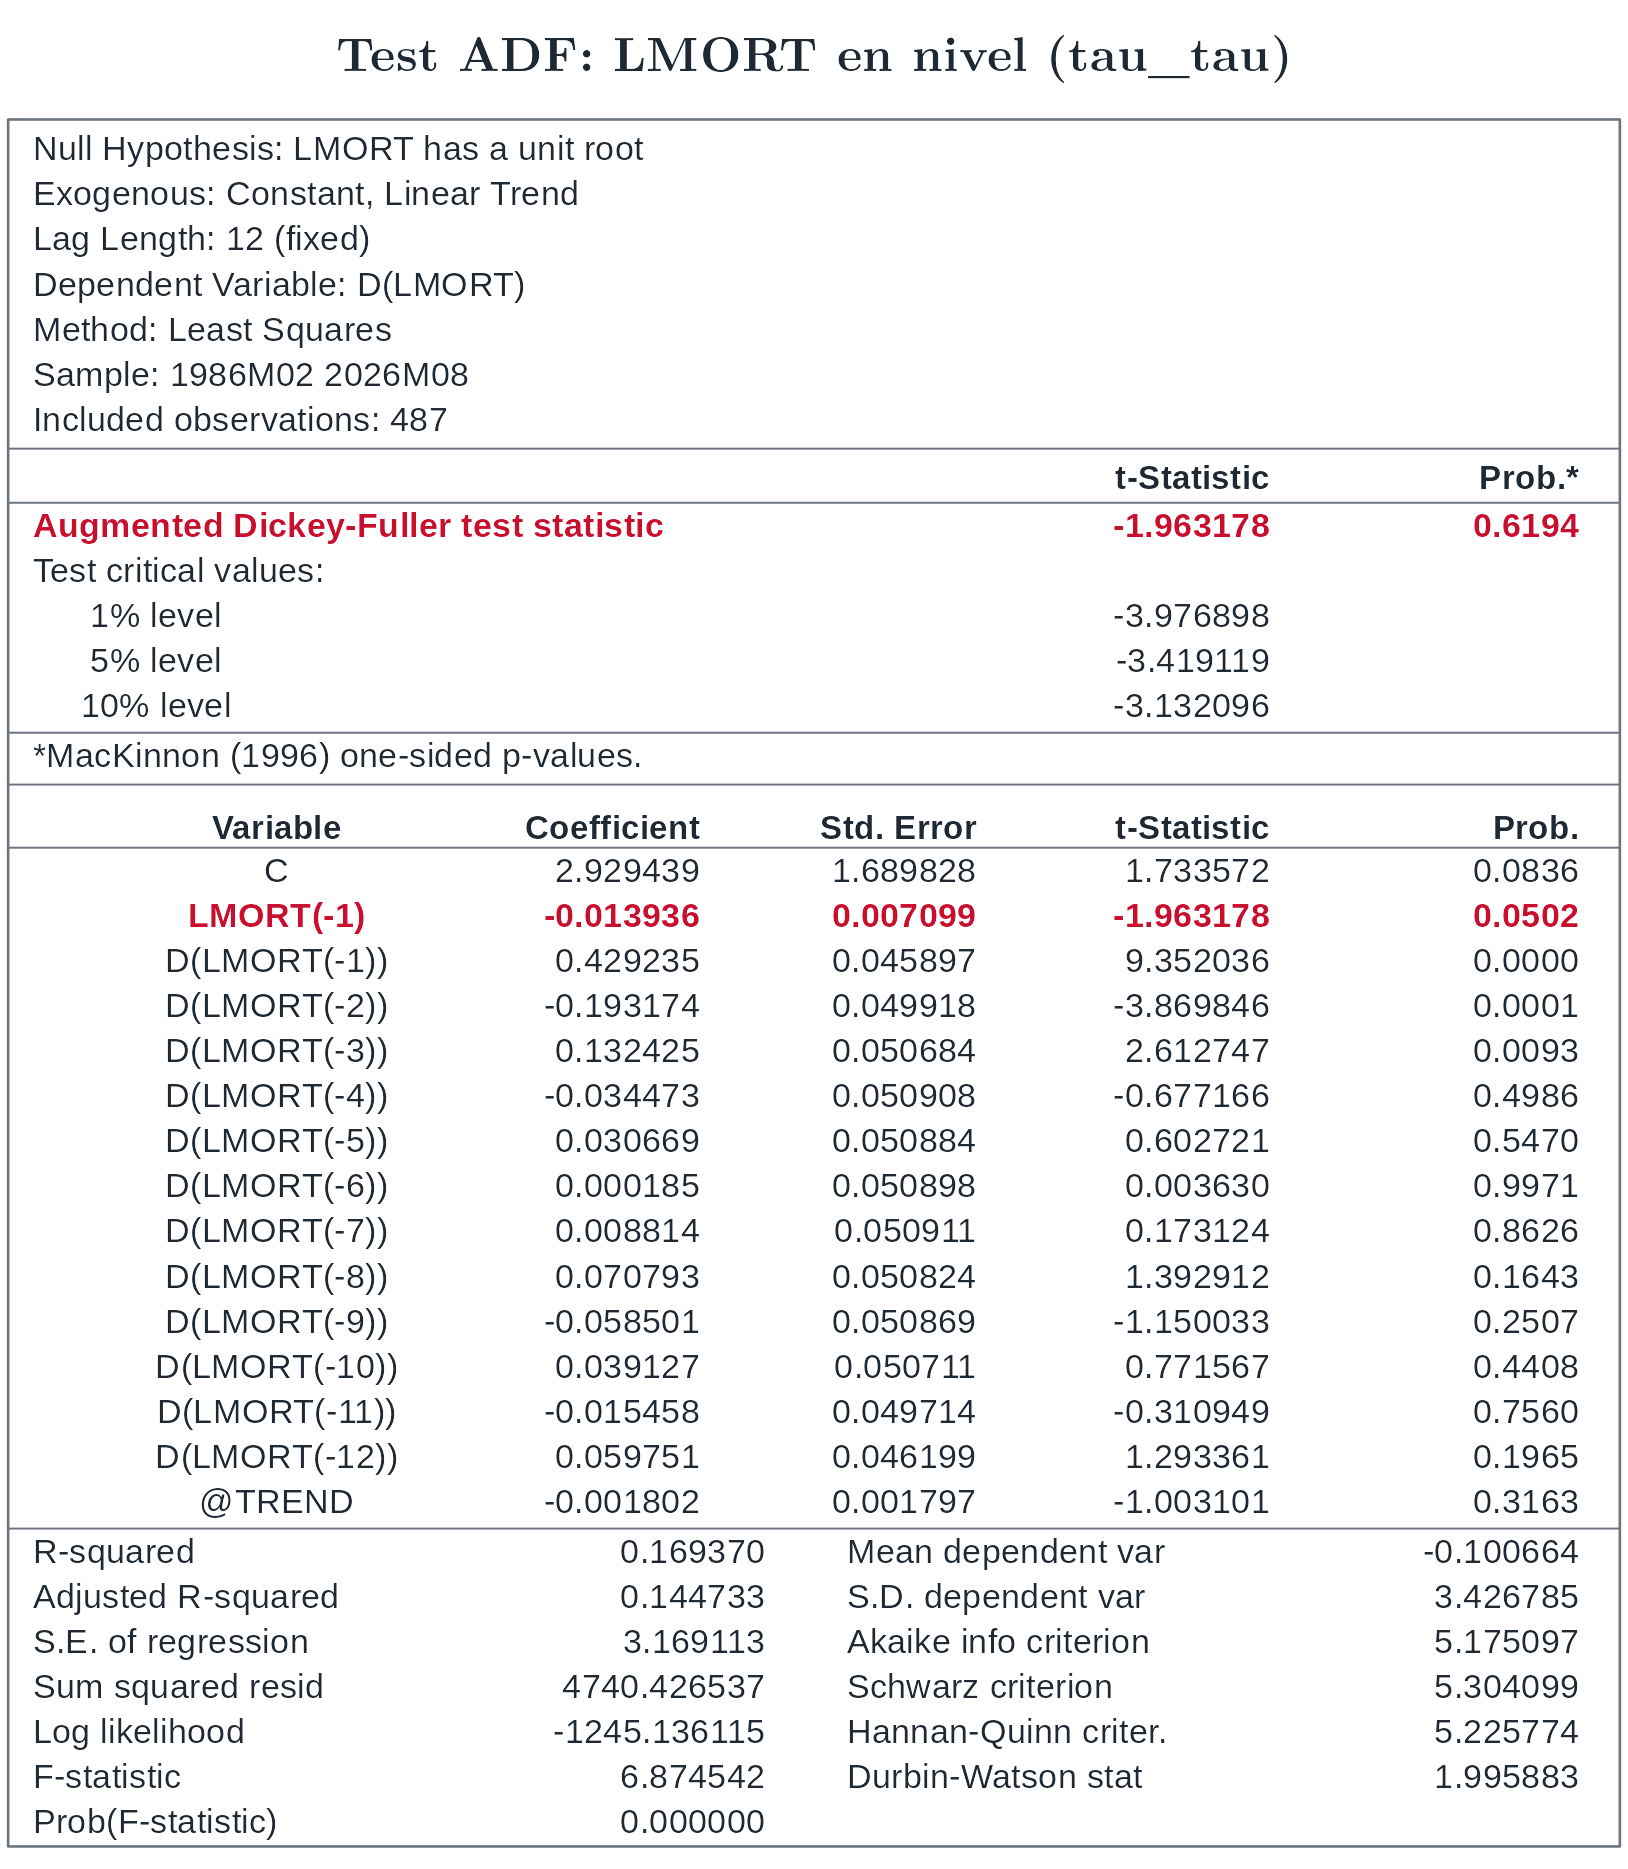
\includegraphics[width=0.49\linewidth]{03_adf_lmort.png}\hfill
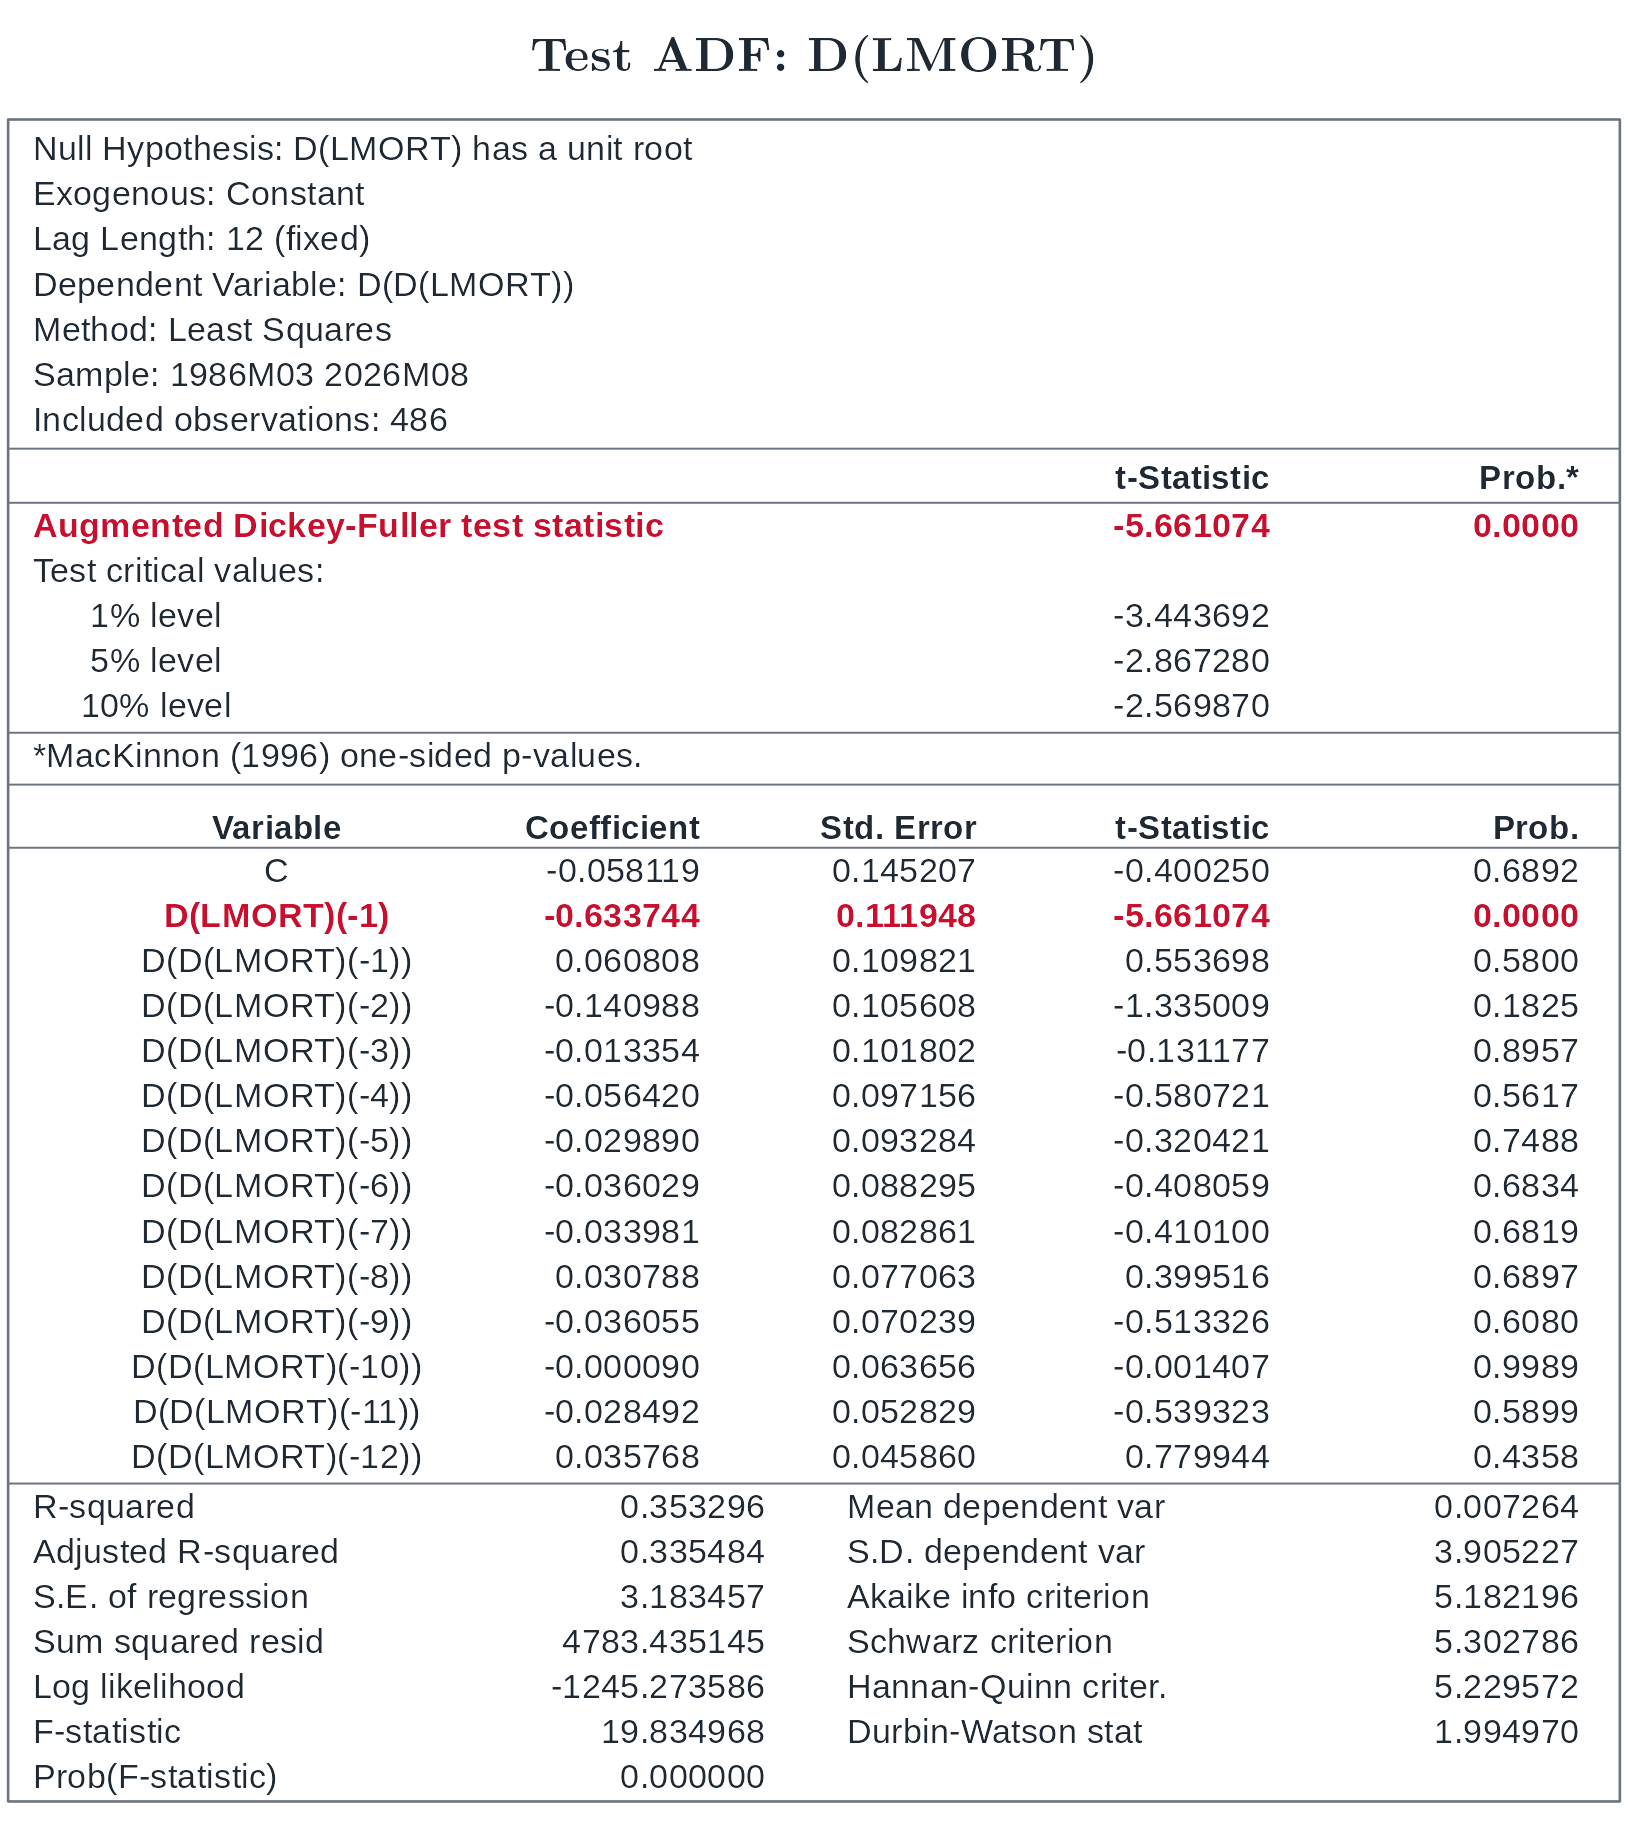
\includegraphics[width=0.49\linewidth]{03_adf_dlmort.png}
\caption{ADF de la tasa: nivel ($\tau_\tau$) y primera diferencia.}
\end{figure}
\begin{figure}[H]\centering
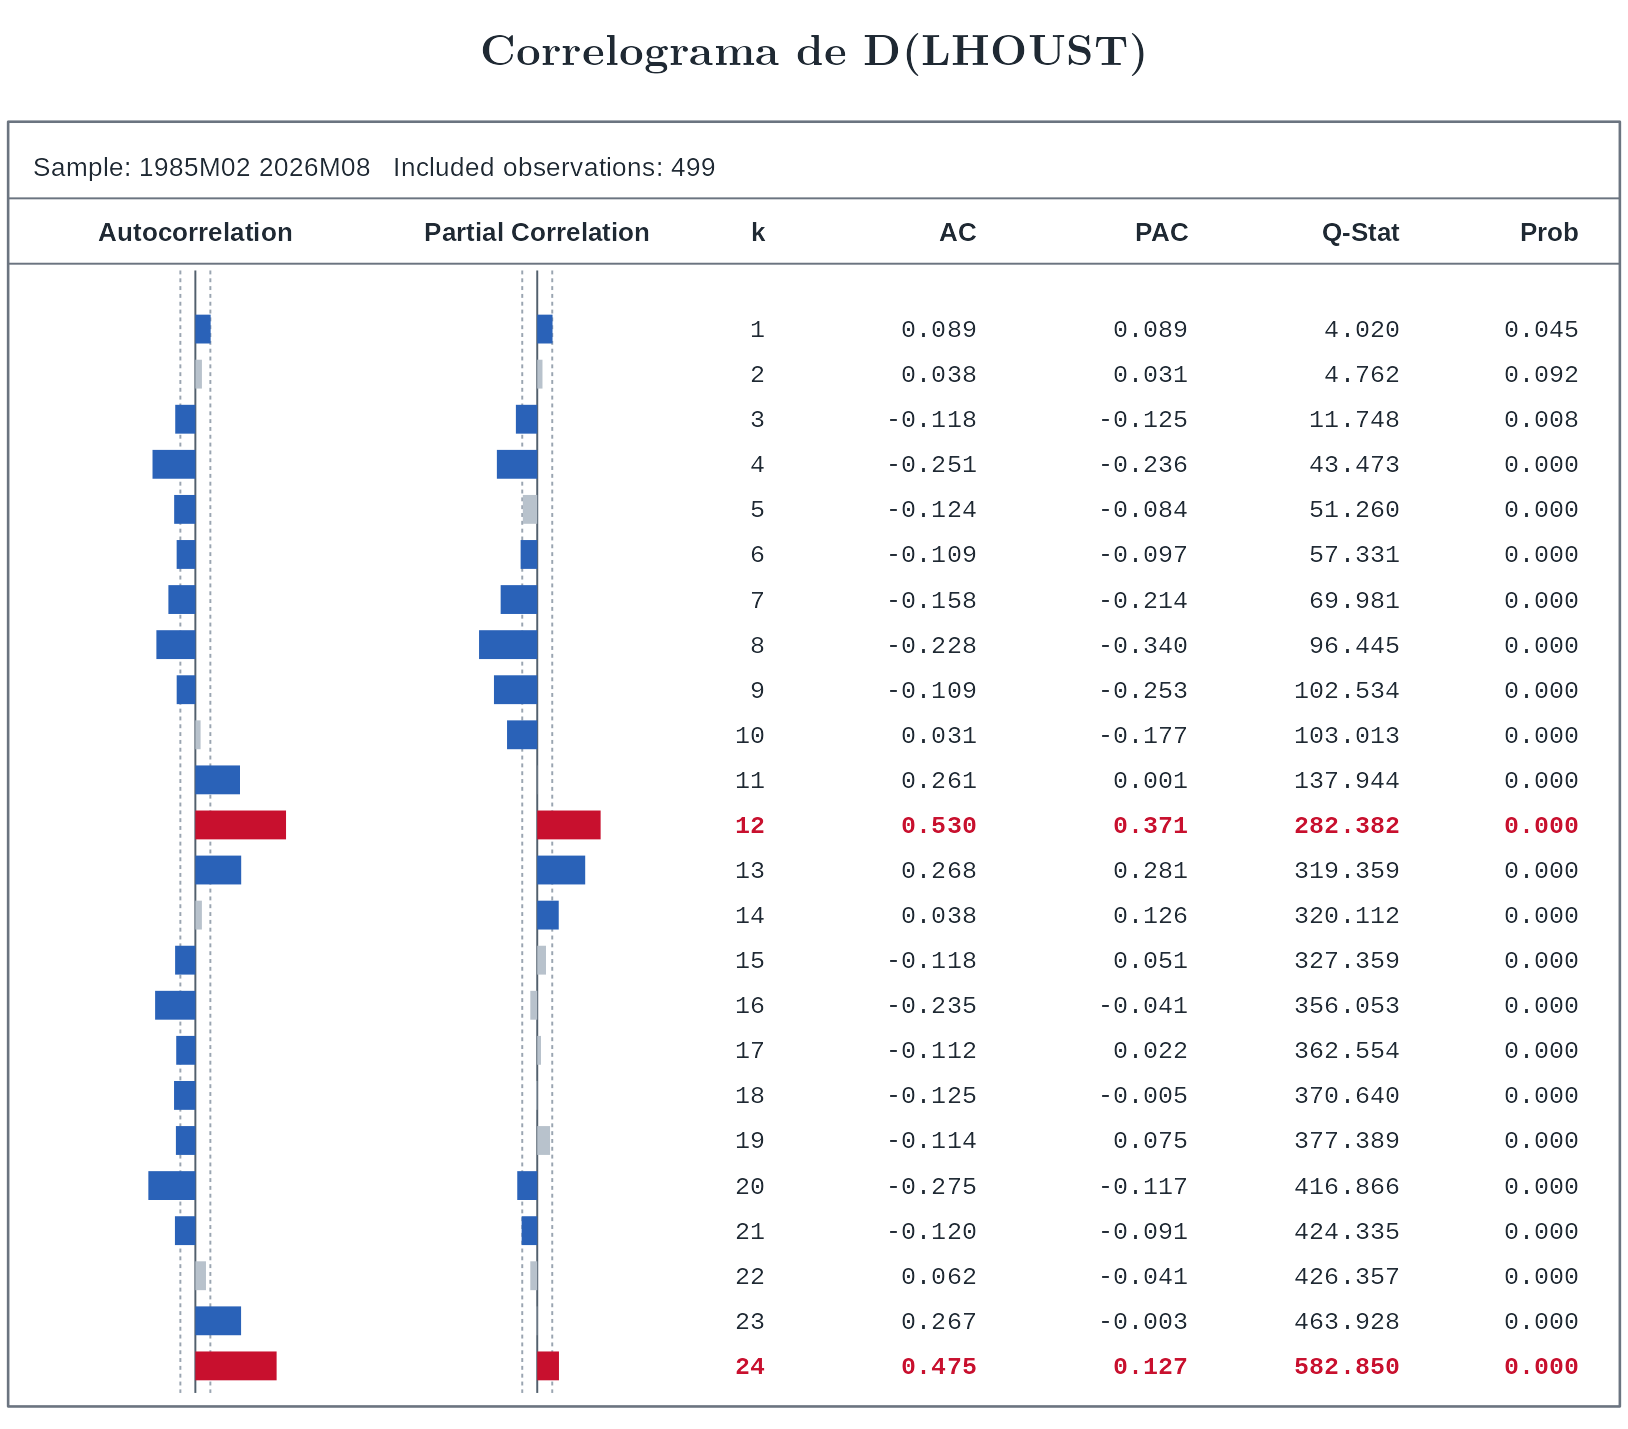
\includegraphics[width=0.49\linewidth]{03_corr_dlhoust.png}\hfill
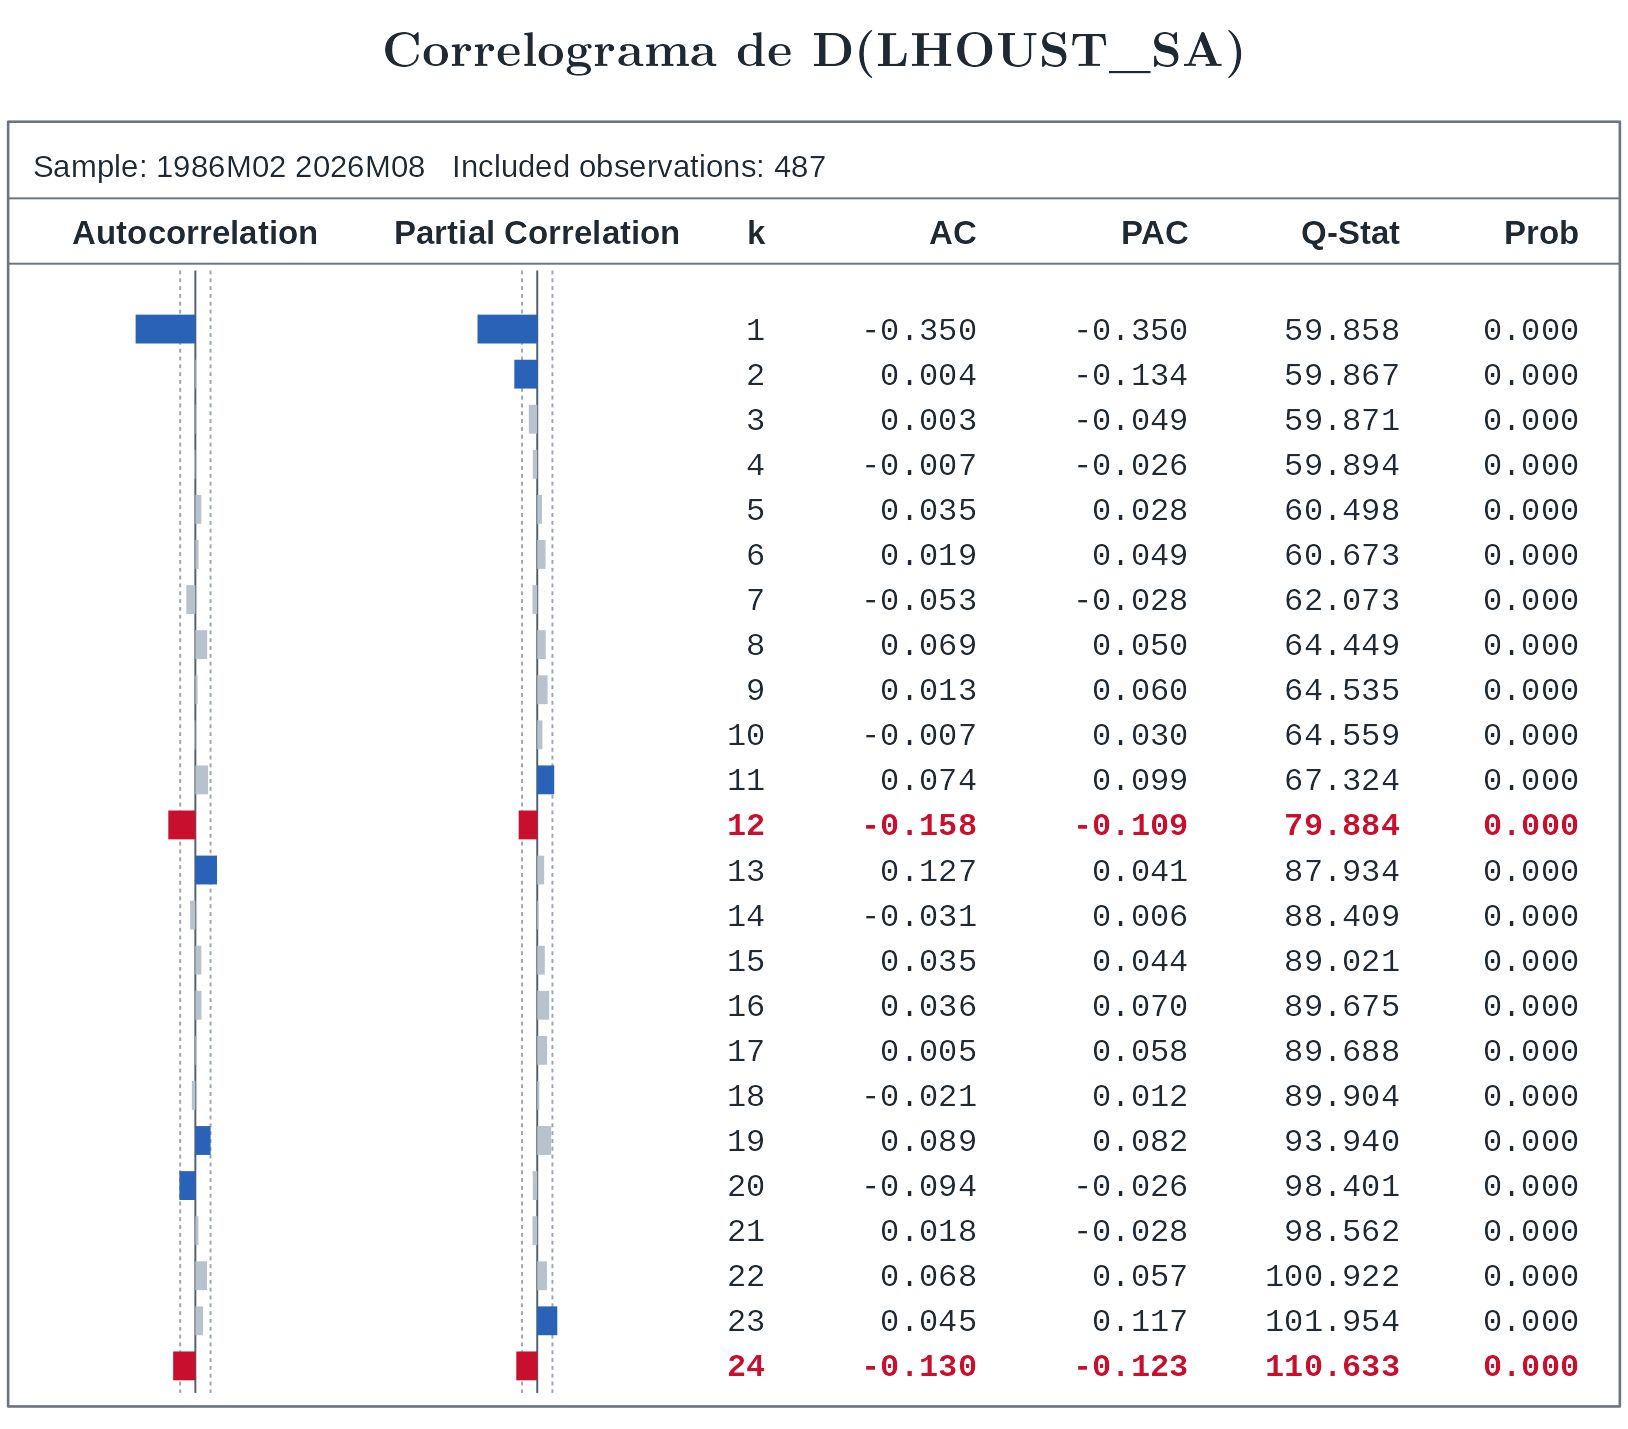
\includegraphics[width=0.49\linewidth]{04_corr_sa.png}
\caption{Correlogramas de $(1-B)x$ (picos estacionales que no decaen) y de la serie desestacionalizada en diferencia.}
\end{figure}
\salida{04_modelo_sa.png}{0.8}{Modelo de la serie desestacionalizada (comparaci\'on, regla 8).}

\end{document}
